\documentclass[11pt, a4paper]{article}

% -- Packages -----------------------------------------------------
\usepackage[utf8]{inputenc}
\usepackage[T1]{fontenc}
\usepackage{lmodern}
\usepackage[margin=2.4cm]{geometry}
\usepackage[table]{xcolor}
\usepackage{amsmath, amssymb, amsthm}
\usepackage{enumitem}
\usepackage{booktabs}
\usepackage{colortbl}
\usepackage{tikz}
\usepackage{tcolorbox}
\usepackage{hyperref}
\usepackage{titlesec}
\usepackage{caption}
\usepackage{float}
\usepackage{pgfplots}
\pgfplotsset{compat=1.18}
\usepgfplotslibrary{groupplots}


\tcbuselibrary{skins, breakable}
\usetikzlibrary{arrows.meta, positioning, calc}

% -- Colors -------------------------------------------------------
\definecolor{accentblue}{RGB}{30, 90, 160}
\definecolor{lightblue}{RGB}{220, 235, 252}
\definecolor{secgray}{RGB}{90, 90, 90}

\definecolor{cache}{RGB}{34, 139, 34}
\definecolor{cachebg}{RGB}{232, 245, 232}
\definecolor{boundary}{RGB}{180, 130, 0}
\definecolor{boundarybg}{RGB}{255, 248, 225}
\definecolor{regular}{RGB}{200, 40, 40}
\definecolor{regularbg}{RGB}{255, 232, 232}

\definecolor{newcolor}{RGB}{210, 85, 15}
\definecolor{newbg}{RGB}{255, 238, 222}
\definecolor{paperbg}{RGB}{228, 238, 252}
\definecolor{felnerbg}{RGB}{240, 232, 248}
\definecolor{felner}{RGB}{100, 50, 150}

% -- Styling ------------------------------------------------------
\hypersetup{
    colorlinks=true,
    linkcolor=accentblue,
    citecolor=accentblue,
    urlcolor=accentblue,
}

\titleformat{\section}
    {\Large\bfseries\color{accentblue}}{\thesection}{1em}{}
    [\vspace{-4pt}{\color{secgray}\titlerule[0.4pt]}]

\titleformat{\subsection}
    {\large\bfseries\color{accentblue!80!black}}{\thesubsection}{1em}{}

\titleformat{\subsubsection}
    {\normalsize\bfseries\color{accentblue!70!black}}{\thesubsubsection}{1em}{}

% -- Enumerated sentences -----------------------------------------
\newlist{sentences}{enumerate}{1}
\setlist[sentences]{
    label=\textbf{\color{accentblue}(\arabic*)},
    leftmargin=2.4em,
    itemsep=3pt,
    parsep=0pt,
    topsep=4pt,
}

% -- Origin tags --------------------------------------------------
\newcommand{\tagours}{%
    {\footnotesize\colorbox{newbg}{%
    \textcolor{newcolor}{\textsf{\textbf{Ours}}}}}%
}
\newcommand{\tagfelner}{%
    {\footnotesize\colorbox{felnerbg}{%
    \textcolor{felner}{\textsf{\textbf{Felner 2011}}}}}%
}

% -- Step badge (for numbered cascade steps) ----------------------
\newcommand{\stepbadge}[1]{%
    \tikz[baseline=(X.base)]%
    \node[circle, fill=regular, text=white,
          font=\bfseries\scriptsize,
          minimum size=0.42cm, inner sep=0pt] (X) {#1};%
}

% ================================================================

% -- Author annotations (draft only) -------------
\newif\ifdraft\drafttrue
\newcommand{\me}[1]{%
    \ifdraft\textcolor{red}{\textbf{[me:\,#1]}}\fi%
}
\newcommand{\you}[1]{%
    \ifdraft\textcolor{blue}{\textbf{[you:\,#1]}}\fi%
}


% -- Insights callout box --
\newtcolorbox{insights}{%
    enhanced, breakable,
    colback=lightblue, colframe=accentblue,
    coltitle=white, fonttitle=\bfseries\small,
    title=Insights, fontupper=\small,
    boxrule=0.4pt, arc=2pt,
    left=6pt, right=6pt, top=3pt, bottom=3pt,
    before skip=8pt, after skip=10pt,
}

\begin{document}
% ================================================================

% -- Title Block --------------------------------------------------
\begin{center}
    {\LARGE\bfseries\color{accentblue}
    MOSPP}

    \vspace{8pt}
    {\large Heuristic Propagation\\[2pt]
    Connection to BPMX}

\end{center}

\vspace{16pt}

% ================================================================
\section{Bidirectional Pathmax (BPMX)}
\hfill\tagfelner
% ================================================================

\paragraph{What is BPMX?}

A heuristic-propagation algorithm that bounds $h$-values
on inconsistent heuristics using the
\textbf{triangle inequality}. BPMX is the cascading
combination of Rules~1 and~3 (Felner et~al., 2011),
depth-bounded by parameter~$d$. The three pathmax rules
below are the building blocks; the BPMX cascade is
defined after them.\\[2pt]
\textit{Notation:}\;\; $p$ = parent,\;\; $c$ = child,\;\;
$d$ = edge distance,\;\; $g$ = goal.

\paragraph{The three pathmax rules
(Felner numbering).}

\begin{sentences}
\item \textbf{Rule 1 --- Pathmax} (Mero, 1984): tighten
      child from parent (``path'' + ``max''):
      \[
          h'(c) = \max\bigl(h(c),\; h(p) - d\bigr).
      \]

      \begin{center}
      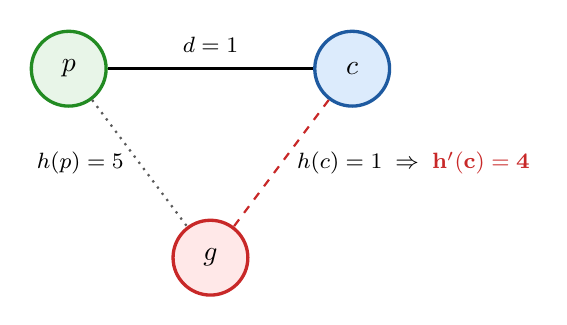
\begin{tikzpicture}[
          nd/.style={circle, minimum size=0.95cm,
                     very thick, font=\bfseries,
                     inner sep=0pt},
      ]
      \node[nd, fill=cachebg, draw=cache] (p)
          at (0, 0) {$p$};
      \node[nd, fill=lightblue, draw=accentblue] (c)
          at (3.6, 0) {$c$};
      \node[nd, fill=regularbg, draw=regular] (g)
          at (1.8, -2.4) {$g$};
      \draw[very thick]
          (p) -- node[above=2pt, font=\footnotesize]
          {$d = 1$} (c);
      \draw[dotted, thick, color=secgray] (p) --
          node[midway, left=2pt, font=\footnotesize,
          color=black]
          {$h(p) = 5$} (g);
      \draw[dashed, thick, color=regular] (c) --
          node[midway, right=2pt, font=\footnotesize,
          color=black]
          {$h(c) = 1 \;\Rightarrow\;
          \textcolor{regular}{\mathbf{h'(c) = 4}}$} (g);
      \end{tikzpicture}
      \end{center}

\item \textbf{Rule 2 --- Min-of-children}
      (Felner et~al., 2011): tighten parent from the
      minimum-cost child. Limited utility when Rules~1
      and~3 are both used (Felner~\S5.4.1).
      \textbf{Depth-1 only by structural constraint:}
      Rule~2's operator consumes \emph{a parent and its
      full children set} and aggregates via $\min$. Chained
      application would require treating the lifted parent
      as a child of its grandparent, but Rule~2 expects to
      receive ``a parent + complete children set'' at each
      invocation, not ``a single child''. The grandparent's
      children set does not include the lifted parent's
      siblings, so the operation has no chained-grandparent
      analogue. Rule~2 is therefore not part of the BPMX
      cascade (which composes Rules~1 and~3 only) and
      cannot be extended to depth $d > 1$ as a standalone
      mechanism. Formally:
      \[
          h'(p) = \max\bigl(h(p),\;
                  \min_{i}\bigl(h(c_i) + d_i\bigr)\bigr).
      \]

      \begin{center}
      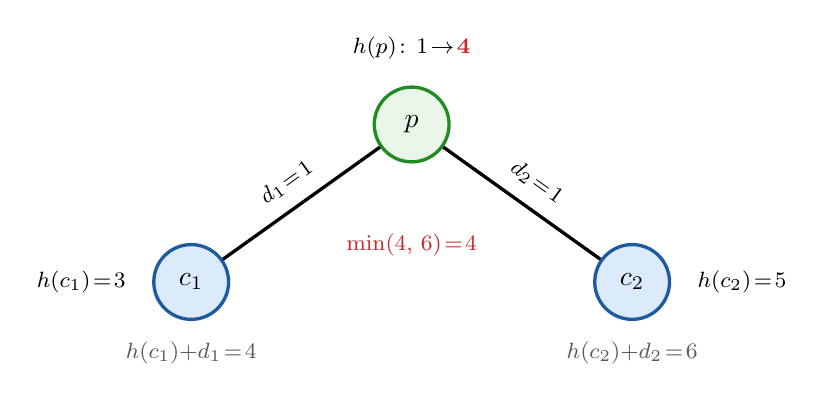
\begin{tikzpicture}[
          nd/.style={circle, minimum size=0.95cm,
                     very thick, font=\bfseries,
                     inner sep=0pt},
          hlab/.style={font=\footnotesize},
      ]
      \node[nd, fill=cachebg, draw=cache] (p)
          at (0, 0) {$p$};
      \node[nd, fill=lightblue, draw=accentblue] (c1)
          at (-2.8, -2.0) {$c_1$};
      \node[nd, fill=lightblue, draw=accentblue] (c2)
          at (2.8, -2.0)  {$c_2$};

      % h-value annotations
      \node[hlab, above=6pt of p]
          {$h(p)\!:\,1\!\to\!%
           \textcolor{regular}{\mathbf{4}}$};
      \node[hlab, left=6pt of c1]
          {$h(c_1)\!=\!3$};
      \node[hlab, right=6pt of c2]
          {$h(c_2)\!=\!5$};

      % Tree edges with d labels
      \draw[very thick] (p) -- node[sloped,
          above=2pt, font=\footnotesize]
          {$d_1\!=\!1$} (c1);
      \draw[very thick] (p) -- node[sloped,
          above=2pt, font=\footnotesize]
          {$d_2\!=\!1$} (c2);

      % Min-of-children annotation
      \node[font=\footnotesize, color=secgray,
            below=4pt of c1, anchor=north]
          {$h(c_1){+}d_1\!=\!4$};
      \node[font=\footnotesize, color=secgray,
            below=4pt of c2, anchor=north]
          {$h(c_2){+}d_2\!=\!6$};
      \node[font=\footnotesize\bfseries,
            color=regular, below=22pt of p]
          {$\min(4,\,6)\!=\!4$};
      \end{tikzpicture}
      \end{center}

\item \textbf{Rule 3 --- Reverse pathmax}
      (Felner et~al., 2011): tighten parent from a
      single child --- the upward counterpart of
      Rule~1, the step that makes pathmax
      \textbf{bidirectional}:
      \[
          h'(p) = \max\bigl(h(p),\; h(c) - d\bigr).
      \]

      \begin{center}
      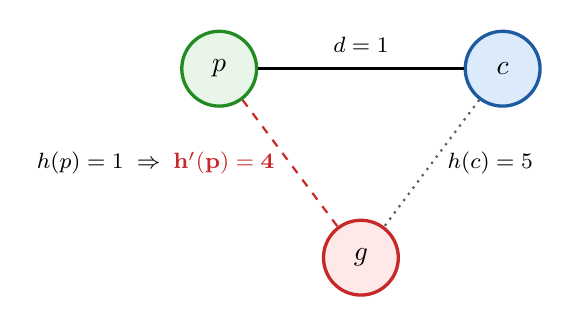
\begin{tikzpicture}[
          nd/.style={circle, minimum size=0.95cm,
                     very thick, font=\bfseries,
                     inner sep=0pt},
      ]
      \node[nd, fill=cachebg, draw=cache] (p)
          at (0, 0) {$p$};
      \node[nd, fill=lightblue, draw=accentblue] (c)
          at (3.6, 0) {$c$};
      \node[nd, fill=regularbg, draw=regular] (g)
          at (1.8, -2.4) {$g$};
      \draw[very thick]
          (p) -- node[above=2pt, font=\footnotesize]
          {$d = 1$} (c);
      \draw[dashed, thick, color=regular] (p) --
          node[midway, left=2pt, font=\footnotesize,
          color=black]
          {$h(p) = 1 \;\Rightarrow\;
          \textcolor{regular}{\mathbf{h'(p) = 4}}$} (g);
      \draw[dotted, thick, color=secgray] (c) --
          node[midway, right=2pt, font=\footnotesize,
          color=black]
          {$h(c) = 5$} (g);
      \end{tikzpicture}
      \end{center}
\end{sentences}

\paragraph{BPMX = Rules~1 + 3 cascading
(Felner Algorithm~2).}
At each expansion of node~$p$ with children
$\{c_i\}$: \textbf{Rule~3} lifts $h(p)$ from a
high-$h$ child; if $h(p)$ is lifted, \textbf{Rule~1}
propagates the new value to every other child~$c'$:
\[
    h'(c') = \max\bigl(h(c'),\; h'(p) - d\bigr).
\]
The cascade extends outward up to depth~$d$ (denoted
BPMX($d$)) or until no node is improved in the last
layer.

\begin{center}
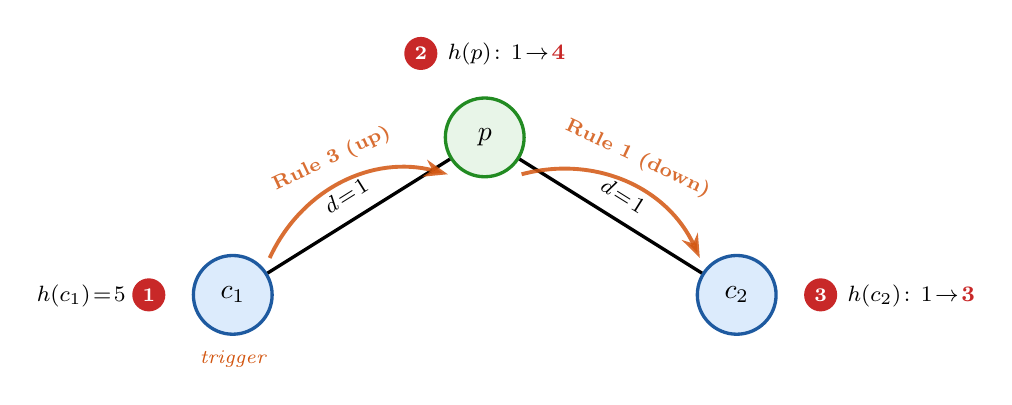
\begin{tikzpicture}[
    nd/.style={circle, minimum size=1.0cm,
               very thick, font=\bfseries,
               inner sep=0pt},
    cascarr/.style={->, line width=1.4pt,
                    color=newcolor,
                    >={Stealth[length=3mm,
                               width=2.2mm]},
                    opacity=0.85},
    hlab/.style={font=\footnotesize},
]

% -- Nodes ----------------------------------
\node[nd, fill=cachebg, draw=cache]
    (p)  at (0, 0)       {$p$};
\node[nd, fill=lightblue, draw=accentblue]
    (c1) at (-3.2, -2.0) {$c_1$};
\node[nd, fill=lightblue, draw=accentblue]
    (c2) at (3.2, -2.0)  {$c_2$};

% -- h-value annotations (step-badged) ------
\node[hlab, above=6pt of p]
    {\stepbadge{2}\;\,%
     $h(p)\!:\,1\!\to\!%
     \textcolor{regular}{\mathbf{4}}$};
\node[hlab, left=6pt of c1]
    {$h(c_1)\!=\!5$\;\stepbadge{1}};
\node[hlab, right=6pt of c2]
    {\stepbadge{3}\;\,%
     $h(c_2)\!:\,1\!\to\!%
     \textcolor{regular}{\mathbf{3}}$};

% -- Trigger marker under c1 -----------------
\node[font=\scriptsize\itshape,
      color=newcolor, below=2pt of c1]
    {trigger};

% -- Tree edges ------------------------------
\draw[very thick] (p) -- node[sloped,
    above=2pt, font=\footnotesize]
    {$d\!=\!1$} (c1);
\draw[very thick] (p) -- node[sloped,
    above=2pt, font=\footnotesize]
    {$d\!=\!1$} (c2);

% -- Cascade-flow overlay arrows -------------
% (1) Rule 3: c1 upward to p
\draw[cascarr]
    ($(c1.north east)+(0.1,0.1)$)
    to[bend left=40]
    node[pos=0.5, sloped, above=2pt,
         font=\scriptsize\bfseries,
         color=newcolor]
    {Rule 3 (up)}
    ($(p.south west)+(-0.1,-0.1)$);

% (2) Rule 1: p downward to c2
\draw[cascarr]
    ($(p.south east)+(0.1,-0.1)$)
    to[bend left=40]
    node[pos=0.5, sloped, above=2pt,
         font=\scriptsize\bfseries,
         color=newcolor]
    {Rule 1 (down)}
    ($(c2.north west)+(-0.1,0.1)$);

\end{tikzpicture}
\end{center}

% -- 1.1 Detailed Example -----------------------------------
\subsection{Detailed Example: BPMX($d{=}2$) Cascade}

\paragraph{Reading the example.}
\begin{sentences}
\item In this example $A$ has the highest $h$ in its
      local neighborhood, so \textbf{Rule~3 (upward)
      does not fire} --- no child can lift $h(A)$. The
      BPMX cascade therefore reduces to a pure
      \textbf{Rule~1 (downward) propagation} of
      depth~2 from $A$ to its descendants.
\item For an example where Rule~3 (upward) does fire
      and triggers downward Rule~1, see the BPMX
      cascade diagram above (with $c_1$ as trigger).
\end{sentences}

\vspace{6pt}

\begin{center}
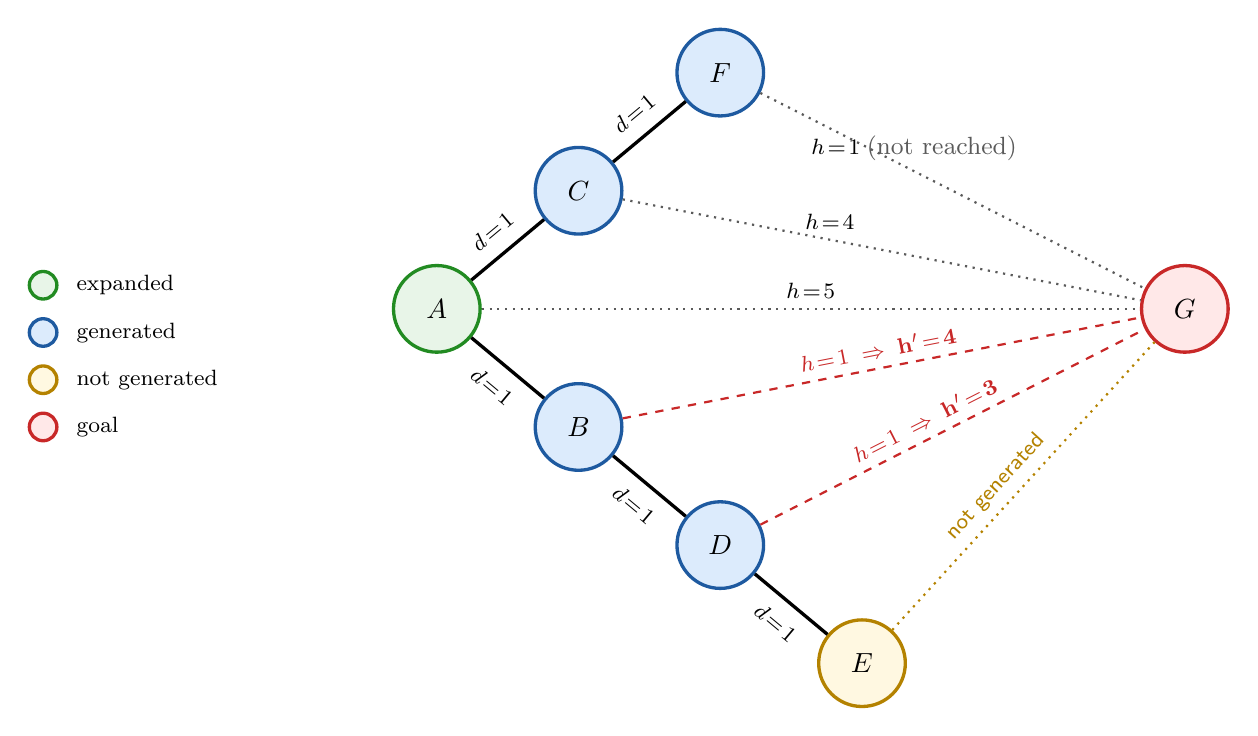
\begin{tikzpicture}[
    nd/.style={circle, minimum size=1.1cm, very thick,
               font=\bfseries, inner sep=0pt},
]

% -- Legend (vertical, left side) --
\begin{scope}[xshift=-5cm, yshift=-0.6cm]
    \node[circle, fill=cachebg, draw=cache,
          very thick, minimum size=0.35cm,
          inner sep=0pt] at (0, 0.9) {};
    \node[right, font=\footnotesize] at (0.3, 0.9)
        {expanded};
    \node[circle, fill=lightblue, draw=accentblue,
          very thick, minimum size=0.35cm,
          inner sep=0pt] at (0, 0.3) {};
    \node[right, font=\footnotesize] at (0.3, 0.3)
        {generated};
    \node[circle, fill=boundarybg, draw=boundary,
          very thick, minimum size=0.35cm,
          inner sep=0pt] at (0, -0.3) {};
    \node[right, font=\footnotesize] at (0.3, -0.3)
        {not generated};
    \node[circle, fill=regularbg, draw=regular,
          very thick, minimum size=0.35cm,
          inner sep=0pt] at (0, -0.9) {};
    \node[right, font=\footnotesize] at (0.3, -0.9)
        {goal};
\end{scope}

% -- Nodes --
\node[nd, fill=cachebg, draw=cache] (A)
    at (0, 0) {$A$};
\node[nd, fill=lightblue, draw=accentblue] (C)
    at (1.8, 1.5) {$C$};
\node[nd, fill=lightblue, draw=accentblue] (F)
    at (3.6, 3.0) {$F$};
\node[nd, fill=lightblue, draw=accentblue] (B)
    at (1.8, -1.5) {$B$};
\node[nd, fill=lightblue, draw=accentblue] (D)
    at (3.6, -3.0) {$D$};
\node[nd, fill=boundarybg, draw=boundary] (E)
    at (5.4, -4.5) {$E$};
\node[nd, fill=regularbg, draw=regular] (G)
    at (9.5, 0) {$G$};

% -- Graph edges (solid, labels perpendicular) --
\draw[very thick]
    (A) -- node[sloped, above=2pt,
    font=\footnotesize] {$d\!=\!1$} (C);
\draw[very thick]
    (C) -- node[sloped, above=2pt,
    font=\footnotesize] {$d\!=\!1$} (F);
\draw[very thick]
    (A) -- node[sloped, below=2pt,
    font=\footnotesize] {$d\!=\!1$} (B);
\draw[very thick]
    (B) -- node[sloped, below=2pt,
    font=\footnotesize] {$d\!=\!1$} (D);
\draw[very thick]
    (D) -- node[sloped, below=2pt,
    font=\footnotesize] {$d\!=\!1$} (E);

% -- Heuristic lines to G (unchanged) --
\draw[dotted, thick, color=secgray]
    (A) -- node[above, font=\footnotesize,
    color=black, pos=0.5] {$h\!=\!5$} (G);
\draw[dotted, thick, color=secgray]
    (C) -- node[above, font=\footnotesize,
    color=black, pos=0.4] {$h\!=\!4$} (G);
\draw[dotted, thick, color=secgray]
    (F) -- node[above, font=\footnotesize,
    color=black, pos=0.4]
    {$h\!=\!1$\;\textcolor{secgray}{\small(not
    reached)}} (G);

% -- BPMX-improved lines (red dashed) --
\draw[dashed, thick, color=regular]
    (B) -- node[above, font=\footnotesize,
    sloped, pos=0.5]
    {$h\!=\!1 \;\Rightarrow\;
    \textcolor{regular}{\mathbf{h'\!=\!4}}$} (G);
\draw[dashed, thick, color=regular]
    (D) -- node[above, font=\footnotesize,
    sloped, pos=0.45]
    {$h\!=\!1 \;\Rightarrow\;
    \textcolor{regular}{\mathbf{h'\!=\!3}}$} (G);

% -- E to G (not generated, dotted) --
\draw[dotted, thick, color=boundary]
    (E) -- node[above, font=\footnotesize,
    color=boundary, sloped, pos=0.45]
    {\textsf{not generated}} (G);

\end{tikzpicture}
\end{center}

\vspace{6pt}

\paragraph{Example.}
\begin{sentences}
\item $A$ is expanded ($h\!=\!5$). Its children $C$
      and $B$ are generated.
\item $C$: $\max(4,\;5\!-\!1) = 4$, no improvement
      (value unchanged). Cascade \textbf{stops} at~$C$.
\item $F$: would improve
      ($\max(1,\;4\!-\!1)=3$), but cascade stopped
      at~$C$ --- deferred to $C$'s expansion.
\item $B$: $\max(1,\;5\!-\!1) = 4$, improved.
      Cascade continues.
\item $D$: $\max(1,\;4\!-\!1) = 3$, improved.
\item $E$: not generated --- cascade stops.
\end{sentences}

\vspace{6pt}

\paragraph{How can inconsistency arise in heuristic search?}
\begin{sentences}
\item[\tagfelner] Random PDB selection, dual state
      heuristic, compressed PDBs, Interleaved
      Differential Heuristics (IDH).
\item In MOSPP: mixing cached $h^*$ with
      regular $h$ across sequential searches.
\end{sentences}

\vspace{8pt}

% -- Comparison Summary --------------------------------------
\subsection{Comparison Summary}

\vspace{4pt}

\begin{table}[H]
\centering
\renewcommand{\arraystretch}{1.6}
\begin{tabular}{l p{4.8cm} p{4.8cm}}
\toprule
& \textbf{HS for OMSPP \& MOSPP}
& \textbf{Inconsistent Heuristics}
  \;\tagfelner \\
\midrule
\rowcolor{accentblue!25}
\textbf{Mechanism}
    & \multicolumn{2}{c}{\textbf{Same: triangle
      inequality on adjacent nodes}} \\
\textbf{Context}
    & $k$ sequential A* searches to
      shared target~$t$
    & Single A* or IDA* search \\
\rowcolor{black!5}
\textbf{Source value}
    & $h^*$ --- exact distance, cached
      from a previous search
    & $h$ --- admissible estimate from
      inconsistent heuristic (random PDB
      selection, dual state lookup,
      compressed PDB, IDH) \\
\textbf{Inconsistency}
    & Localized at cached/uncached
      boundary; structurally predictable
    & Distributed across the graph;
      location-unpredictable \\
\rowcolor{black!5}
\textbf{Timing}
    & Pre-propagation between searches
    & Online during node expansion \\
\textbf{Depth}
    & Tunable parameter~$d$
      ($d\!=\!2$ empirically best),
      \textbf{or} adaptive: stop when no
      node was improved in the last
      propagation step
    & BPMX($d$): $d\!=\!1$ to $\infty$;
      stops when value no longer improves
      neighbors \\
\rowcolor{black!5}
\textbf{Beyond}
    & Early termination: cached node
      expanded $\Rightarrow$ path
      reconstruction
    & Value propagation only \\
\bottomrule
\end{tabular}
\end{table}

\vspace{8pt}
\section{Heuristic-Reuse Mechanisms: Adaptive, Propagation, BPMX}
% ================================================================

\paragraph{Three mechanisms, one shared store.}

The incremental orchestrator strengthens the inner heuristic by
three independent mechanisms. Two are \textbf{sources} (they
originate new admissible bounds); two are \textbf{spreaders}
(they extend existing bounds to further nodes). All three write
the \emph{same} admissible \texttt{HBounded} layer and combine
by~$\max$, so they stack freely and A* optimality is preserved.

\paragraph{The three mechanisms.}

\begin{sentences}
\item \textbf{Adaptive heuristic} (\emph{source};
      Koenig \& Likhachev, 2005): after a sub-search solves
      start $s_i$ with optimal cost $C_i$, set
      \[
          h(x) \leftarrow \max\bigl(h(x),\; C_i - g_i(x)\bigr)
          \quad\text{for every expanded } x,
      \]
      admissible since $C_i \le g_i(x) + h^*(x, t)$. Turns each
      solved start into a landmark; covers \emph{all}
      previously expanded nodes (on- and off-path); free --- a
      by-product of the closed list. Intrinsically cross-search.
      Knob: \texttt{adaptive\_h}.

\item \textbf{Heuristic propagation} (\emph{spreader}, eager):
      before a sub-search, pathmax is propagated outward from
      already-elevated nodes (cache and carried bounds) to
      \texttt{propagate\_depth} levels. Spreads known
      information; originates none, so on a cold first search it
      does nothing. Pays a one-off pre-search cost over a
      region. Knobs: \texttt{propagate}, \texttt{propagate\_depth}.

\item \textbf{BPMX} (\emph{spreader}, lazy; Felner et~al.,
      2011): during search, the pathmax cascade runs on the BFS
      subtree around each expanded node. Spreads rather than
      originates, but lazily, on the live frontier, paying per
      expansion only where the search goes. Knobs:
      \texttt{rule\_bpmx}, \texttt{depth\_bpmx}.
\end{sentences}

\begin{table}[H]
\centering
\small
\begin{tabular}{@{}llll@{}}
\toprule
\textbf{Mechanism} & \textbf{Role} & \textbf{When} & \textbf{Covers} \\
\midrule
Adaptive    & source   & cross-search & every expanded node \\
Propagation & spreader & pre-search   & seeds $+$ depth-neighbours \\
BPMX        & spreader & in-search    & live-frontier subtree \\
\bottomrule
\end{tabular}
\caption{Sources originate admissible bounds; spreaders extend
them. The three write one shared \texttt{HBounded} layer and
compose by~$\max$.}
\end{table}

\paragraph{Can they be combined?}

Yes. Every bound is an admissible lower bound on $h^*(x, t)$, so
their $\max$ is admissible and A* optimality holds under any
combination; co-active propagation~$+$~BPMX is verified in the
unit tests. The three are orthogonal knobs on one shared store,
not competing alternatives.

\paragraph{When is each beneficial?}

\begin{sentences}
\item \textbf{Adaptive} --- whenever later sub-searches revisit
      regions earlier searches expanded. Pays most when the base
      heuristic is \emph{loose} (obstacles, weights, detours)
      and adds nothing when the base is already exact (open grid
      with Manhattan, where $C_i - g_i(x) \le \text{Manhattan}$
      always).
\item \textbf{Propagation} --- when the current search enters
      \emph{new} territory adjacent to known bounds; the cheap
      global informer that carries the cache/adaptive bounds
      into the unexplored neighbourhood.
\item \textbf{BPMX} --- only when a live inconsistency exists in
      territory neither cached nor propagated; the expensive
      local option. Prefer propagation; reach for BPMX when
      propagation is depth-capped and residual inconsistency
      remains.
      \me{why should i always prefer propagation over bpmx in MOSPP? what bpmx rule is best for MOSPP?}
      \you{Because in MOSPP all inconsistency originates in the carried cache/bounds (the base Manhattan $h$ is consistent) and is known before the sub-search, propagation spreads it once pre-search whereas BPMX re-derives the same lifts per expansion (wall-clock rose about $10\times$ with depth in our runs); it is not literally always---reach for \texttt{rule\_bpmx=1} at \texttt{depth=2} (the 44\% expansion drop) only for residual inconsistency that propagation's depth cap misses.}
\item \textbf{First sub-search} --- none help (no prior $C_i$,
      no seeds, consistent base): it is plain A*.
\item \textbf{Static graph (MOSPP)} --- edge costs never change,
      so the adaptive update needs only basic Adaptive A*, never
      the cost-change correction of Generalized Adaptive A*.
\end{sentences}

\vspace{8pt}

% ====================================================================
%  Experimental results -- per-rule sections generated by s_5.
%  Do NOT hand-edit rule1/rule2/rule3/cascade.tex; edit
%  report_spec.py / report_render.py instead. This main.tex
%  (preamble + sections 1-2 + the \input list) is human-owned.
% ====================================================================
\IfFileExists{rule1.tex}{\section{Experimental Results --- BPMX Rule 1 depth ladder}

\subsection{Mean |Expanded Nodes| per k.}
\begin{figure}[H]
\centering
\includegraphics{fig_rule1_cnt_expanded}
\caption{Line chart.}
\end{figure}


\begin{table}[H]
\centering
\caption{Data results.}
\small
\setlength{\tabcolsep}{6pt}
\begin{tabular}{lrrrrr}
\toprule
\textbf{depth} & \textbf{$k{=}10$} & \textbf{$k{=}50$} & \textbf{$k{=}100$} & \textbf{$k{=}150$} & \textbf{$k{=}200$} \\
\midrule
  depth=0 & \cellcolor[HTML]{F8696B}113,538 & \cellcolor[HTML]{F8696B}217,159 & \cellcolor[HTML]{F8696B}257,358 & \cellcolor[HTML]{F8696B}274,123 & \cellcolor[HTML]{F8696B}285,235 \\
  depth=1 & \cellcolor[HTML]{F8696B}113,538 & \cellcolor[HTML]{F8696B}217,159 & \cellcolor[HTML]{F8696B}257,358 & \cellcolor[HTML]{F8696B}274,123 & \cellcolor[HTML]{F8696B}285,235 \\
  depth=2 & \cellcolor[HTML]{81C77D}70,505 & \cellcolor[HTML]{7FC67D}119,995 & \cellcolor[HTML]{87C87D}145,600 & \cellcolor[HTML]{88C97D}156,972 & \cellcolor[HTML]{83C77D}160,306 \\
  depth=3 & \cellcolor[HTML]{6EC17C}67,632 & \cellcolor[HTML]{6BC07B}113,246 & \cellcolor[HTML]{79C47C}140,027 & \cellcolor[HTML]{79C47C}150,675 & \cellcolor[HTML]{77C47C}154,867 \\
  depth=4 & \cellcolor[HTML]{64BE7B}66,159 & \cellcolor[HTML]{65BF7B}111,087 & \cellcolor[HTML]{65BF7B}132,046 & \cellcolor[HTML]{65BF7B}142,264 & \cellcolor[HTML]{65BF7B}147,126 \\
  depth=5 & \cellcolor[HTML]{63BE7B}65,934 & \cellcolor[HTML]{63BE7B}110,466 & \cellcolor[HTML]{63BE7B}131,211 & \cellcolor[HTML]{63BE7B}141,375 & \cellcolor[HTML]{63BE7B}146,114 \\
\bottomrule
\end{tabular}
\end{table}


\begin{insights}
\begin{sentences}
\item $d{=}0$ and $d{=}1$ are identical -- a depth-1 sweep lifts nothing on consistent~$h$.
\item The largest drop is $d{=}1\to d{=}2$ ($\approx 1.8\times$).
\item Expansions keep falling with depth, but the gains diminish past $d{=}2$.
\end{sentences}
\end{insights}


\subsection{Mean |BPMX Attempts| per k.}
\begin{figure}[H]
\centering
\includegraphics{fig_rule1_cnt_bpmx_attempts}
\caption{Line chart.}
\end{figure}


\begin{table}[H]
\centering
\caption{Data results.}
\small
\setlength{\tabcolsep}{6pt}
\begin{tabular}{lrrrrr}
\toprule
\textbf{depth} & \textbf{$k{=}10$} & \textbf{$k{=}50$} & \textbf{$k{=}100$} & \textbf{$k{=}150$} & \textbf{$k{=}200$} \\
\midrule
  depth=0 & \cellcolor[HTML]{63BE7B}0 & \cellcolor[HTML]{63BE7B}0 & \cellcolor[HTML]{63BE7B}0 & \cellcolor[HTML]{63BE7B}0 & \cellcolor[HTML]{63BE7B}0 \\
  depth=1 & \cellcolor[HTML]{F8696B}113,538 & \cellcolor[HTML]{F8696B}217,159 & \cellcolor[HTML]{F8696B}257,358 & \cellcolor[HTML]{F8696B}274,123 & \cellcolor[HTML]{F8696B}285,235 \\
  depth=2 & \cellcolor[HTML]{FDCC7E}70,505 & \cellcolor[HTML]{FEDD81}119,995 & \cellcolor[HTML]{FEDA81}145,600 & \cellcolor[HTML]{FED880}156,972 & \cellcolor[HTML]{FEDB81}160,306 \\
  depth=3 & \cellcolor[HTML]{FED27F}67,632 & \cellcolor[HTML]{FFE583}113,246 & \cellcolor[HTML]{FEE082}140,027 & \cellcolor[HTML]{FEDE82}150,675 & \cellcolor[HTML]{FEE082}154,867 \\
  depth=4 & \cellcolor[HTML]{FED580}66,159 & \cellcolor[HTML]{FFE883}111,087 & \cellcolor[HTML]{FFE883}132,046 & \cellcolor[HTML]{FFE683}142,264 & \cellcolor[HTML]{FFE783}147,126 \\
  depth=5 & \cellcolor[HTML]{FED680}65,934 & \cellcolor[HTML]{FFE984}110,466 & \cellcolor[HTML]{FFE884}131,211 & \cellcolor[HTML]{FFE783}141,375 & \cellcolor[HTML]{FFE883}146,114 \\
\bottomrule
\end{tabular}
\end{table}


\begin{insights}
\begin{sentences}
\item $d{=}0$: no BPMX attempts (BPMX is off).
\item $d{\ge}1$: attempts equal the expanded-node count -- one sweep per expansion.
\end{sentences}
\end{insights}


\subsection{Mean |BPMX Lifts| per k.}
\begin{figure}[H]
\centering
\includegraphics{fig_rule1_cnt_bpmx_lifts}
\caption{Line chart.}
\end{figure}


\begin{table}[H]
\centering
\caption{Data results.}
\small
\setlength{\tabcolsep}{6pt}
\begin{tabular}{lrrrrr}
\toprule
\textbf{depth} & \textbf{$k{=}10$} & \textbf{$k{=}50$} & \textbf{$k{=}100$} & \textbf{$k{=}150$} & \textbf{$k{=}200$} \\
\midrule
  depth=0 & \cellcolor[HTML]{63BE7B}0 & \cellcolor[HTML]{63BE7B}0 & \cellcolor[HTML]{63BE7B}0 & \cellcolor[HTML]{63BE7B}0 & \cellcolor[HTML]{63BE7B}0 \\
  depth=1 & \cellcolor[HTML]{63BE7B}0 & \cellcolor[HTML]{63BE7B}0 & \cellcolor[HTML]{63BE7B}0 & \cellcolor[HTML]{63BE7B}0 & \cellcolor[HTML]{63BE7B}0 \\
  depth=2 & \cellcolor[HTML]{F8716D}18,415 & \cellcolor[HTML]{F86C6C}43,376 & \cellcolor[HTML]{F8696B}55,303 & \cellcolor[HTML]{F8696B}56,978 & \cellcolor[HTML]{F8696B}57,950 \\
  depth=3 & \cellcolor[HTML]{FA9574}15,759 & \cellcolor[HTML]{FA9774}36,078 & \cellcolor[HTML]{F98170}50,174 & \cellcolor[HTML]{F98270}51,393 & \cellcolor[HTML]{F98170}52,567 \\
  depth=4 & \cellcolor[HTML]{FA8C72}16,439 & \cellcolor[HTML]{FA8871}38,606 & \cellcolor[HTML]{FA8871}48,724 & \cellcolor[HTML]{FA8971}50,030 & \cellcolor[HTML]{FA8871}50,981 \\
  depth=5 & \cellcolor[HTML]{F8696B}19,008 & \cellcolor[HTML]{F8696B}43,821 & \cellcolor[HTML]{F86C6B}54,762 & \cellcolor[HTML]{F86C6B}56,416 & \cellcolor[HTML]{F86A6B}57,689 \\
\bottomrule
\end{tabular}
\end{table}


\begin{insights}
\begin{sentences}
\item $d{\le}1$: no lifts.
\item $d{\ge}2$: small spread, no monotonic pattern across depths.
\end{sentences}
\end{insights}


\subsection{Mean \%(BPMX Lifts / Attempts) per k.}
\begin{figure}[H]
\centering
\includegraphics{fig_rule1_pct_bpmx_lifts}
\caption{Line chart.}
\end{figure}


\begin{table}[H]
\centering
\caption{Data results.}
\small
\setlength{\tabcolsep}{6pt}
\begin{tabular}{lrrrrr}
\toprule
\textbf{depth} & \textbf{$k{=}10$} & \textbf{$k{=}50$} & \textbf{$k{=}100$} & \textbf{$k{=}150$} & \textbf{$k{=}200$} \\
\midrule
  depth=0 & \cellcolor[HTML]{63BE7B}0\% & \cellcolor[HTML]{63BE7B}0\% & \cellcolor[HTML]{63BE7B}0\% & \cellcolor[HTML]{63BE7B}0\% & \cellcolor[HTML]{63BE7B}0\% \\
  depth=1 & \cellcolor[HTML]{63BE7B}0\% & \cellcolor[HTML]{63BE7B}0\% & \cellcolor[HTML]{63BE7B}0\% & \cellcolor[HTML]{63BE7B}0\% & \cellcolor[HTML]{63BE7B}0\% \\
  depth=2 & \cellcolor[HTML]{FCB77A}11.07\% & \cellcolor[HTML]{FDBE7B}13.83\% & \cellcolor[HTML]{FDC67D}14.79\% & \cellcolor[HTML]{FCBC7B}15.96\% & \cellcolor[HTML]{FCB079}17.00\% \\
  depth=3 & \cellcolor[HTML]{FCAE78}11.67\% & \cellcolor[HTML]{FCAE78}15.07\% & \cellcolor[HTML]{FCAD78}16.96\% & \cellcolor[HTML]{FCAB78}17.48\% & \cellcolor[HTML]{FB9E75}18.60\% \\
  depth=4 & \cellcolor[HTML]{FB9874}13.00\% & \cellcolor[HTML]{FA9173}17.38\% & \cellcolor[HTML]{FA9073}19.55\% & \cellcolor[HTML]{FA9273}19.69\% & \cellcolor[HTML]{FA9173}19.75\% \\
  depth=5 & \cellcolor[HTML]{F8696B}15.84\% & \cellcolor[HTML]{F8696B}20.54\% & \cellcolor[HTML]{F8696B}23.01\% & \cellcolor[HTML]{F8696B}23.41\% & \cellcolor[HTML]{F8696B}23.33\% \\
\bottomrule
\end{tabular}
\end{table}


\begin{insights}
\begin{sentences}
\item $d{\le}1$: no lifts, so the rate is $0\%$.
\item $d{\ge}2$: the hit-rate rises monotonically with depth.
\end{sentences}
\end{insights}


\subsection{\texttt{mem\_open}}
\begin{figure}[H]
\centering
\includegraphics{fig_rule1_mem_open}
\caption{Line chart.}
\end{figure}


\begin{table}[H]
\centering
\caption{Data results.}
\small
\setlength{\tabcolsep}{6pt}
\begin{tabular}{lrrrrr}
\toprule
\textbf{depth} & \textbf{$k{=}10$} & \textbf{$k{=}50$} & \textbf{$k{=}100$} & \textbf{$k{=}150$} & \textbf{$k{=}200$} \\
\midrule
  depth=0 & \cellcolor[HTML]{F8696B}160,063 & \cellcolor[HTML]{F8696B}164,506 & \cellcolor[HTML]{F8696B}165,856 & \cellcolor[HTML]{F8696B}165,856 & \cellcolor[HTML]{F8696B}165,856 \\
  depth=1 & \cellcolor[HTML]{F8696B}160,063 & \cellcolor[HTML]{F8696B}164,506 & \cellcolor[HTML]{F8696B}165,856 & \cellcolor[HTML]{F8696B}165,856 & \cellcolor[HTML]{F8696B}165,856 \\
  depth=2 & \cellcolor[HTML]{87C87D}147,503 & \cellcolor[HTML]{AFD47F}152,165 & \cellcolor[HTML]{BED880}155,289 & \cellcolor[HTML]{BCD880}155,289 & \cellcolor[HTML]{BCD880}155,289 \\
  depth=3 & \cellcolor[HTML]{63BE7B}145,870 & \cellcolor[HTML]{91CB7E}150,598 & \cellcolor[HTML]{B6D680}154,920 & \cellcolor[HTML]{B4D580}154,920 & \cellcolor[HTML]{B4D580}154,920 \\
  depth=4 & \cellcolor[HTML]{E7E483}151,866 & \cellcolor[HTML]{FFE783}156,582 & \cellcolor[HTML]{FED880}159,464 & \cellcolor[HTML]{FED981}159,464 & \cellcolor[HTML]{FED981}159,464 \\
  depth=5 & \cellcolor[HTML]{80C67D}147,183 & \cellcolor[HTML]{63BE7B}148,179 & \cellcolor[HTML]{63BE7B}150,934 & \cellcolor[HTML]{63BE7B}151,081 & \cellcolor[HTML]{63BE7B}151,081 \\
\bottomrule
\end{tabular}
\end{table}


\begin{insights}
\begin{sentences}
\item Per-sub-search peak OPEN size (bytes), aggregated across the $k$ sub-searches.
\end{sentences}
\end{insights}


\subsection{\texttt{mem\_closed}}
\begin{figure}[H]
\centering
\includegraphics{fig_rule1_mem_closed}
\caption{Line chart.}
\end{figure}


\begin{table}[H]
\centering
\caption{Data results.}
\small
\setlength{\tabcolsep}{6pt}
\begin{tabular}{lrrrrr}
\toprule
\textbf{depth} & \textbf{$k{=}10$} & \textbf{$k{=}50$} & \textbf{$k{=}100$} & \textbf{$k{=}150$} & \textbf{$k{=}200$} \\
\midrule
  depth=0 & 5,571,775 & 5,572,168 & 5,572,474 & 5,572,474 & 5,572,474 \\
  depth=1 & 5,571,775 & 5,572,168 & 5,572,474 & 5,572,474 & 5,572,474 \\
  depth=2 & 5,571,775 & 5,572,168 & 5,572,474 & 5,572,474 & 5,572,474 \\
  depth=3 & 5,571,775 & 5,572,168 & 5,572,474 & 5,572,474 & 5,572,474 \\
  depth=4 & 5,571,775 & 5,572,168 & 5,572,474 & 5,572,474 & 5,572,474 \\
  depth=5 & 5,571,775 & 5,572,168 & 5,572,474 & 5,572,474 & 5,572,474 \\
\bottomrule
\end{tabular}
\end{table}


\begin{insights}
\begin{sentences}
\item Per-sub-search peak CLOSED size (bytes), aggregated across the $k$ sub-searches.
\end{sentences}
\end{insights}


\subsection{\texttt{mem\_total}}
\begin{figure}[H]
\centering
\includegraphics{fig_rule1_mem_total}
\caption{Line chart.}
\end{figure}


\begin{table}[H]
\centering
\caption{Data results.}
\small
\setlength{\tabcolsep}{6pt}
\begin{tabular}{lrrrrr}
\toprule
\textbf{depth} & \textbf{$k{=}10$} & \textbf{$k{=}50$} & \textbf{$k{=}100$} & \textbf{$k{=}150$} & \textbf{$k{=}200$} \\
\midrule
  depth=0 & \cellcolor[HTML]{F8696B}5,866,594 & \cellcolor[HTML]{F8696B}5,936,732 & \cellcolor[HTML]{F8696B}5,962,686 & \cellcolor[HTML]{F8696B}5,970,732 & \cellcolor[HTML]{F8696B}5,989,624 \\
  depth=1 & \cellcolor[HTML]{F8696B}5,866,594 & \cellcolor[HTML]{F8696B}5,936,732 & \cellcolor[HTML]{F8696B}5,962,686 & \cellcolor[HTML]{F8696B}5,970,732 & \cellcolor[HTML]{F8696B}5,989,624 \\
  depth=2 & \cellcolor[HTML]{90CB7E}5,844,608 & \cellcolor[HTML]{ADD37F}5,911,091 & \cellcolor[HTML]{95CC7E}5,941,510 & \cellcolor[HTML]{8FCB7E}5,951,909 & \cellcolor[HTML]{7AC57C}5,957,024 \\
  depth=3 & \cellcolor[HTML]{71C27C}5,842,001 & \cellcolor[HTML]{7AC57C}5,905,541 & \cellcolor[HTML]{84C77D}5,940,129 & \cellcolor[HTML]{7BC57C}5,950,488 & \cellcolor[HTML]{72C27C}5,956,153 \\
  depth=4 & \cellcolor[HTML]{AAD37F}5,846,744 & \cellcolor[HTML]{A4D17F}5,910,122 & \cellcolor[HTML]{B1D580}5,943,783 & \cellcolor[HTML]{B2D580}5,954,378 & \cellcolor[HTML]{91CB7E}5,959,697 \\
  depth=5 & \cellcolor[HTML]{63BE7B}5,840,861 & \cellcolor[HTML]{63BE7B}5,903,098 & \cellcolor[HTML]{63BE7B}5,937,474 & \cellcolor[HTML]{63BE7B}5,948,814 & \cellcolor[HTML]{63BE7B}5,954,471 \\
\bottomrule
\end{tabular}
\end{table}


\begin{insights}
\begin{sentences}
\item Sum of every memory region per sub-search: OPEN $+$ CLOSED $+$ cache $+$ bounds.
\end{sentences}
\end{insights}


\subsection{Mean Runtime (in seconds) per k}
\begin{figure}[H]
\centering
\includegraphics{fig_rule1_elapsed_total}
\caption{Line chart.}
\end{figure}


\begin{table}[H]
\centering
\caption{Data results.}
\small
\setlength{\tabcolsep}{6pt}
\begin{tabular}{lrrrrr}
\toprule
\textbf{depth} & \textbf{$k{=}10$} & \textbf{$k{=}50$} & \textbf{$k{=}100$} & \textbf{$k{=}150$} & \textbf{$k{=}200$} \\
\midrule
  depth=0 & \cellcolor[HTML]{63BE7B}6.83 & \cellcolor[HTML]{63BE7B}11.75 & \cellcolor[HTML]{63BE7B}13.62 & \cellcolor[HTML]{63BE7B}14.44 & \cellcolor[HTML]{63BE7B}14.99 \\
  depth=1 & \cellcolor[HTML]{81C77D}13.64 & \cellcolor[HTML]{84C87D}23.18 & \cellcolor[HTML]{85C87D}26.80 & \cellcolor[HTML]{84C87D}28.34 & \cellcolor[HTML]{85C87D}29.38 \\
  depth=2 & \cellcolor[HTML]{91CB7E}17.44 & \cellcolor[HTML]{90CB7E}27.02 & \cellcolor[HTML]{91CB7E}31.66 & \cellcolor[HTML]{91CB7E}33.70 & \cellcolor[HTML]{91CB7E}34.41 \\
  depth=3 & \cellcolor[HTML]{D0DD81}31.79 & \cellcolor[HTML]{CDDD81}48.05 & \cellcolor[HTML]{D1DE81}56.60 & \cellcolor[HTML]{D1DE81}60.06 & \cellcolor[HTML]{D0DE81}61.63 \\
  depth=4 & \cellcolor[HTML]{FDC97D}51.89 & \cellcolor[HTML]{FDCA7E}78.78 & \cellcolor[HTML]{FDCA7E}90.20 & \cellcolor[HTML]{FDCA7E}95.73 & \cellcolor[HTML]{FDCA7E}98.52 \\
  depth=5 & \cellcolor[HTML]{F8696B}78.33 & \cellcolor[HTML]{F8696B}118.78 & \cellcolor[HTML]{F8696B}135.63 & \cellcolor[HTML]{F8696B}143.96 & \cellcolor[HTML]{F8696B}147.95 \\
\bottomrule
\end{tabular}
\end{table}


\begin{insights}
\begin{sentences}
\item Runtime rises monotonically with depth.
\item The $d{=}1$ to $d{=}2$ step adds the least.
\end{sentences}
\end{insights}

}{}
\IfFileExists{rule2.tex}{\section{Experimental Results --- BPMX Rule 2 (depth=1)}

\subsection{Mean |Expanded Nodes| per k.}
\begin{figure}[H]
\centering
\includegraphics{fig_rule2_cnt_expanded}
\caption{Line chart.}
\end{figure}


\begin{table}[H]
\centering
\caption{Data results.}
\small
\setlength{\tabcolsep}{6pt}
\begin{tabular}{lrrrrr}
\toprule
\textbf{depth} & \textbf{$k{=}10$} & \textbf{$k{=}50$} & \textbf{$k{=}100$} & \textbf{$k{=}150$} & \textbf{$k{=}200$} \\
\midrule
  depth=0 & 113,538 & 217,159 & 257,358 & 274,123 & 285,235 \\
  depth=1 & 113,538 & 217,159 & 257,358 & 274,123 & 285,235 \\
\bottomrule
\end{tabular}
\end{table}


\begin{insights}
\begin{sentences}
\item $d{=}1$ expands exactly the BPMX-off baseline -- the depth-1 lifts raise $h$ but never enough to prune.
\end{sentences}
\end{insights}


\subsection{Mean |BPMX Attempts| per k.}
\begin{figure}[H]
\centering
\includegraphics{fig_rule2_cnt_bpmx_attempts}
\caption{Line chart.}
\end{figure}


\begin{table}[H]
\centering
\caption{Data results.}
\small
\setlength{\tabcolsep}{6pt}
\begin{tabular}{lrrrrr}
\toprule
\textbf{depth} & \textbf{$k{=}10$} & \textbf{$k{=}50$} & \textbf{$k{=}100$} & \textbf{$k{=}150$} & \textbf{$k{=}200$} \\
\midrule
  depth=0 & \cellcolor[HTML]{63BE7B}0 & \cellcolor[HTML]{63BE7B}0 & \cellcolor[HTML]{63BE7B}0 & \cellcolor[HTML]{63BE7B}0 & \cellcolor[HTML]{63BE7B}0 \\
  depth=1 & \cellcolor[HTML]{F8696B}113,538 & \cellcolor[HTML]{F8696B}217,159 & \cellcolor[HTML]{F8696B}257,358 & \cellcolor[HTML]{F8696B}274,123 & \cellcolor[HTML]{F8696B}285,235 \\
\bottomrule
\end{tabular}
\end{table}


\begin{insights}
\begin{sentences}
\item $d{=}0$: BPMX off. $d{=}1$: one sweep per expansion (equals |Expanded Nodes|).
\end{sentences}
\end{insights}


\subsection{Mean |BPMX Lifts| per k.}
\begin{figure}[H]
\centering
\includegraphics{fig_rule2_cnt_bpmx_lifts}
\caption{Line chart.}
\end{figure}


\begin{table}[H]
\centering
\caption{Data results.}
\small
\setlength{\tabcolsep}{6pt}
\begin{tabular}{lrrrrr}
\toprule
\textbf{depth} & \textbf{$k{=}10$} & \textbf{$k{=}50$} & \textbf{$k{=}100$} & \textbf{$k{=}150$} & \textbf{$k{=}200$} \\
\midrule
  depth=0 & \cellcolor[HTML]{63BE7B}0 & \cellcolor[HTML]{63BE7B}0 & \cellcolor[HTML]{63BE7B}0 & \cellcolor[HTML]{63BE7B}0 & \cellcolor[HTML]{63BE7B}0 \\
  depth=1 & \cellcolor[HTML]{F8696B}7,654 & \cellcolor[HTML]{F8696B}14,425 & \cellcolor[HTML]{F8696B}17,280 & \cellcolor[HTML]{F8696B}18,537 & \cellcolor[HTML]{F8696B}19,292 \\
\bottomrule
\end{tabular}
\end{table}


\begin{insights}
\begin{sentences}
\item $d{=}1$ lifts $h$-values -- unlike Rule 1 (inert at $d{=}1$ on consistent $h$), Rule 2 fires at depth 1.
\item But the lifts never prune: |Expanded| stays at the baseline.
\end{sentences}
\end{insights}


\subsection{Mean \%(BPMX Lifts / Attempts) per k.}
\begin{figure}[H]
\centering
\includegraphics{fig_rule2_pct_bpmx_lifts}
\caption{Line chart.}
\end{figure}


\begin{table}[H]
\centering
\caption{Data results.}
\small
\setlength{\tabcolsep}{6pt}
\begin{tabular}{lrrrrr}
\toprule
\textbf{depth} & \textbf{$k{=}10$} & \textbf{$k{=}50$} & \textbf{$k{=}100$} & \textbf{$k{=}150$} & \textbf{$k{=}200$} \\
\midrule
  depth=0 & \cellcolor[HTML]{63BE7B}0\% & \cellcolor[HTML]{63BE7B}0\% & \cellcolor[HTML]{63BE7B}0\% & \cellcolor[HTML]{63BE7B}0\% & \cellcolor[HTML]{63BE7B}0\% \\
  depth=1 & \cellcolor[HTML]{F8696B}7.28\% & \cellcolor[HTML]{F8696B}7.81\% & \cellcolor[HTML]{F8696B}7.58\% & \cellcolor[HTML]{F8696B}7.72\% & \cellcolor[HTML]{F8696B}7.81\% \\
\bottomrule
\end{tabular}
\end{table}


\begin{insights}
\begin{sentences}
\item $d{=}1$ has a nonzero per-attempt hit-rate -- Rule 2 lifts at depth 1 where Rule 1 does not.
\end{sentences}
\end{insights}


\subsection{\texttt{mem\_open}}
\begin{figure}[H]
\centering
\includegraphics{fig_rule2_mem_open}
\caption{Line chart.}
\end{figure}


\begin{table}[H]
\centering
\caption{Data results.}
\small
\setlength{\tabcolsep}{6pt}
\begin{tabular}{lrrrrr}
\toprule
\textbf{depth} & \textbf{$k{=}10$} & \textbf{$k{=}50$} & \textbf{$k{=}100$} & \textbf{$k{=}150$} & \textbf{$k{=}200$} \\
\midrule
  depth=0 & 160,063 & 164,506 & 165,856 & 165,856 & 165,856 \\
  depth=1 & 160,063 & 164,506 & 165,856 & 165,856 & 165,856 \\
\bottomrule
\end{tabular}
\end{table}


\begin{insights}
\begin{sentences}
\item Per-sub-search peak OPEN size (bytes), aggregated across the $k$ sub-searches.
\end{sentences}
\end{insights}


\subsection{\texttt{mem\_closed}}
\begin{figure}[H]
\centering
\includegraphics{fig_rule2_mem_closed}
\caption{Line chart.}
\end{figure}


\begin{table}[H]
\centering
\caption{Data results.}
\small
\setlength{\tabcolsep}{6pt}
\begin{tabular}{lrrrrr}
\toprule
\textbf{depth} & \textbf{$k{=}10$} & \textbf{$k{=}50$} & \textbf{$k{=}100$} & \textbf{$k{=}150$} & \textbf{$k{=}200$} \\
\midrule
  depth=0 & 5,571,775 & 5,572,168 & 5,572,474 & 5,572,474 & 5,572,474 \\
  depth=1 & 5,571,775 & 5,572,168 & 5,572,474 & 5,572,474 & 5,572,474 \\
\bottomrule
\end{tabular}
\end{table}


\begin{insights}
\begin{sentences}
\item Per-sub-search peak CLOSED size (bytes), aggregated across the $k$ sub-searches.
\end{sentences}
\end{insights}


\subsection{\texttt{mem\_total}}
\begin{figure}[H]
\centering
\includegraphics{fig_rule2_mem_total}
\caption{Line chart.}
\end{figure}


\begin{table}[H]
\centering
\caption{Data results.}
\small
\setlength{\tabcolsep}{6pt}
\begin{tabular}{lrrrrr}
\toprule
\textbf{depth} & \textbf{$k{=}10$} & \textbf{$k{=}50$} & \textbf{$k{=}100$} & \textbf{$k{=}150$} & \textbf{$k{=}200$} \\
\midrule
  depth=0 & 5,866,594 & 5,936,732 & 5,962,686 & 5,970,732 & 5,989,624 \\
  depth=1 & 5,866,594 & 5,936,732 & 5,962,686 & 5,970,732 & 5,989,624 \\
\bottomrule
\end{tabular}
\end{table}


\begin{insights}
\begin{sentences}
\item Sum of every memory region per sub-search.
\end{sentences}
\end{insights}


\subsection{Mean Runtime (in seconds) per k}
\begin{figure}[H]
\centering
\includegraphics{fig_rule2_elapsed_total}
\caption{Line chart.}
\end{figure}


\begin{table}[H]
\centering
\caption{Data results.}
\small
\setlength{\tabcolsep}{6pt}
\begin{tabular}{lrrrrr}
\toprule
\textbf{depth} & \textbf{$k{=}10$} & \textbf{$k{=}50$} & \textbf{$k{=}100$} & \textbf{$k{=}150$} & \textbf{$k{=}200$} \\
\midrule
  depth=0 & \cellcolor[HTML]{63BE7B}6.83 & \cellcolor[HTML]{63BE7B}11.75 & \cellcolor[HTML]{63BE7B}13.62 & \cellcolor[HTML]{63BE7B}14.44 & \cellcolor[HTML]{63BE7B}14.99 \\
  depth=1 & \cellcolor[HTML]{F8696B}10.12 & \cellcolor[HTML]{F8696B}17.25 & \cellcolor[HTML]{F8696B}20.01 & \cellcolor[HTML]{F8696B}21.15 & \cellcolor[HTML]{F8696B}21.94 \\
\bottomrule
\end{tabular}
\end{table}


\begin{insights}
\begin{sentences}
\item $d{=}1$ is slower than the baseline (per-expansion sweep cost) with no expansion savings -- pure overhead here.
\end{sentences}
\end{insights}

}{}
\IfFileExists{rule3.tex}{\section{Experimental Results --- BPMX Rule 3 depth ladder}

\subsection{Mean |Expanded Nodes| per k.}
\begin{figure}[H]
\centering
\includegraphics{fig_rule3_cnt_expanded}
\caption{Line chart.}
\end{figure}


\begin{table}[H]
\centering
\caption{Data results.}
\small
\setlength{\tabcolsep}{6pt}
\begin{tabular}{lrrrrr}
\toprule
\textbf{depth} & \textbf{$k{=}10$} & \textbf{$k{=}50$} & \textbf{$k{=}100$} & \textbf{$k{=}150$} & \textbf{$k{=}200$} \\
\midrule
  depth=0 & \cellcolor[HTML]{F8696B}113,538 & \cellcolor[HTML]{F8696B}217,159 & \cellcolor[HTML]{F8696B}257,358 & \cellcolor[HTML]{F8696B}274,123 & \cellcolor[HTML]{F8696B}285,235 \\
  depth=1 & \cellcolor[HTML]{F8696B}113,538 & \cellcolor[HTML]{F8696B}217,159 & \cellcolor[HTML]{F8696B}257,358 & \cellcolor[HTML]{F8696B}274,123 & \cellcolor[HTML]{F8696B}285,235 \\
  depth=2 & \cellcolor[HTML]{B1D47F}83,424 & \cellcolor[HTML]{BED880}133,219 & \cellcolor[HTML]{C1D980}154,868 & \cellcolor[HTML]{C3DA81}165,654 & \cellcolor[HTML]{C1D980}169,714 \\
  depth=3 & \cellcolor[HTML]{8BC97D}78,513 & \cellcolor[HTML]{7BC57C}107,481 & \cellcolor[HTML]{81C77D}124,816 & \cellcolor[HTML]{82C77D}133,089 & \cellcolor[HTML]{83C77D}136,695 \\
  depth=4 & \cellcolor[HTML]{86C87D}77,979 & \cellcolor[HTML]{77C47C}105,938 & \cellcolor[HTML]{75C37C}118,812 & \cellcolor[HTML]{74C37C}125,990 & \cellcolor[HTML]{74C37C}128,423 \\
  depth=5 & \cellcolor[HTML]{63BE7B}73,415 & \cellcolor[HTML]{63BE7B}98,486 & \cellcolor[HTML]{63BE7B}110,512 & \cellcolor[HTML]{63BE7B}117,490 & \cellcolor[HTML]{63BE7B}119,567 \\
\bottomrule
\end{tabular}
\end{table}


\begin{insights}
\begin{sentences}
\item Inner-A* node expansions, summed across the $k$ sub-searches.
\end{sentences}
\end{insights}


\subsection{Mean |BPMX Attempts| per k.}
\begin{figure}[H]
\centering
\includegraphics{fig_rule3_cnt_bpmx_attempts}
\caption{Line chart.}
\end{figure}


\begin{table}[H]
\centering
\caption{Data results.}
\small
\setlength{\tabcolsep}{6pt}
\begin{tabular}{lrrrrr}
\toprule
\textbf{depth} & \textbf{$k{=}10$} & \textbf{$k{=}50$} & \textbf{$k{=}100$} & \textbf{$k{=}150$} & \textbf{$k{=}200$} \\
\midrule
  depth=0 & \cellcolor[HTML]{63BE7B}0 & \cellcolor[HTML]{63BE7B}0 & \cellcolor[HTML]{63BE7B}0 & \cellcolor[HTML]{63BE7B}0 & \cellcolor[HTML]{63BE7B}0 \\
  depth=1 & \cellcolor[HTML]{F8696B}113,538 & \cellcolor[HTML]{F8696B}217,159 & \cellcolor[HTML]{F8696B}257,358 & \cellcolor[HTML]{F8696B}274,123 & \cellcolor[HTML]{F8696B}285,235 \\
  depth=2 & \cellcolor[HTML]{FCAE78}83,424 & \cellcolor[HTML]{FDCE7E}133,219 & \cellcolor[HTML]{FED17F}154,868 & \cellcolor[HTML]{FED07F}165,654 & \cellcolor[HTML]{FED27F}169,714 \\
  depth=3 & \cellcolor[HTML]{FCB97A}78,513 & \cellcolor[HTML]{FDEB84}107,481 & \cellcolor[HTML]{FAEA84}124,816 & \cellcolor[HTML]{FAEA84}133,089 & \cellcolor[HTML]{F9E984}136,695 \\
  depth=4 & \cellcolor[HTML]{FCBA7B}77,979 & \cellcolor[HTML]{FBEA84}105,938 & \cellcolor[HTML]{F3E883}118,812 & \cellcolor[HTML]{F2E783}125,990 & \cellcolor[HTML]{EFE783}128,423 \\
  depth=5 & \cellcolor[HTML]{FDC57D}73,415 & \cellcolor[HTML]{F0E783}98,486 & \cellcolor[HTML]{E9E583}110,512 & \cellcolor[HTML]{E9E583}117,490 & \cellcolor[HTML]{E6E483}119,567 \\
\bottomrule
\end{tabular}
\end{table}


\begin{insights}
\begin{sentences}
\item BPMX sweeps launched -- one per inner-A* expansion.
\end{sentences}
\end{insights}


\subsection{Mean |BPMX Lifts| per k.}
\begin{figure}[H]
\centering
\includegraphics{fig_rule3_cnt_bpmx_lifts}
\caption{Line chart.}
\end{figure}


\begin{table}[H]
\centering
\caption{Data results.}
\small
\setlength{\tabcolsep}{6pt}
\begin{tabular}{lrrrrr}
\toprule
\textbf{depth} & \textbf{$k{=}10$} & \textbf{$k{=}50$} & \textbf{$k{=}100$} & \textbf{$k{=}150$} & \textbf{$k{=}200$} \\
\midrule
  depth=0 & \cellcolor[HTML]{63BE7B}0 & \cellcolor[HTML]{63BE7B}0 & \cellcolor[HTML]{63BE7B}0 & \cellcolor[HTML]{63BE7B}0 & \cellcolor[HTML]{63BE7B}0 \\
  depth=1 & \cellcolor[HTML]{F8696B}65,573 & \cellcolor[HTML]{F8696B}158,693 & \cellcolor[HTML]{F8696B}193,743 & \cellcolor[HTML]{F8696B}208,612 & \cellcolor[HTML]{F8696B}218,596 \\
  depth=2 & \cellcolor[HTML]{FDC47C}42,740 & \cellcolor[HTML]{FEDB81}89,362 & \cellcolor[HTML]{FED880}110,925 & \cellcolor[HTML]{FED580}121,802 & \cellcolor[HTML]{FED780}126,214 \\
  depth=3 & \cellcolor[HTML]{FDC47D}42,500 & \cellcolor[HTML]{F1E783}72,323 & \cellcolor[HTML]{F6E883}91,001 & \cellcolor[HTML]{F8E984}99,892 & \cellcolor[HTML]{F8E984}104,079 \\
  depth=4 & \cellcolor[HTML]{FDC37C}42,759 & \cellcolor[HTML]{F1E783}72,320 & \cellcolor[HTML]{EFE683}87,108 & \cellcolor[HTML]{F2E783}95,435 & \cellcolor[HTML]{EFE683}98,301 \\
  depth=5 & \cellcolor[HTML]{FDCE7E}40,150 & \cellcolor[HTML]{EAE583}68,829 & \cellcolor[HTML]{E9E583}82,975 & \cellcolor[HTML]{ECE583}91,378 & \cellcolor[HTML]{E9E583}94,063 \\
\bottomrule
\end{tabular}
\end{table}


\begin{insights}
\begin{sentences}
\item BPMX lifts that raised an $h$-value, summed across the $k$ sub-searches.
\end{sentences}
\end{insights}


\subsection{Mean \%(BPMX Lifts / Attempts) per k.}
\begin{figure}[H]
\centering
\includegraphics{fig_rule3_pct_bpmx_lifts}
\caption{Line chart.}
\end{figure}


\begin{table}[H]
\centering
\caption{Data results.}
\small
\setlength{\tabcolsep}{6pt}
\begin{tabular}{lrrrrr}
\toprule
\textbf{depth} & \textbf{$k{=}10$} & \textbf{$k{=}50$} & \textbf{$k{=}100$} & \textbf{$k{=}150$} & \textbf{$k{=}200$} \\
\midrule
  depth=0 & \cellcolor[HTML]{63BE7B}0\% & \cellcolor[HTML]{63BE7B}0\% & \cellcolor[HTML]{63BE7B}0\% & \cellcolor[HTML]{63BE7B}0\% & \cellcolor[HTML]{63BE7B}0\% \\
  depth=1 & \cellcolor[HTML]{FA8F72}25.80\% & \cellcolor[HTML]{FB9A74}35.39\% & \cellcolor[HTML]{FB9C75}38.59\% & \cellcolor[HTML]{FB9E75}40.32\% & \cellcolor[HTML]{FBA076}41.13\% \\
  depth=2 & \cellcolor[HTML]{FA8971}26.51\% & \cellcolor[HTML]{FB9974}35.53\% & \cellcolor[HTML]{FB9A74}38.88\% & \cellcolor[HTML]{FB9B75}40.82\% & \cellcolor[HTML]{FB9A74}42.31\% \\
  depth=3 & \cellcolor[HTML]{F97E6F}27.80\% & \cellcolor[HTML]{F98470}39.06\% & \cellcolor[HTML]{F98370}43.26\% & \cellcolor[HTML]{F98370}45.51\% & \cellcolor[HTML]{F98270}47.13\% \\
  depth=4 & \cellcolor[HTML]{F97F6F}27.69\% & \cellcolor[HTML]{F98370}39.24\% & \cellcolor[HTML]{F97F6F}43.84\% & \cellcolor[HTML]{F97E6F}46.50\% & \cellcolor[HTML]{F97D6F}48.12\% \\
  depth=5 & \cellcolor[HTML]{F8696B}30.19\% & \cellcolor[HTML]{F8696B}43.64\% & \cellcolor[HTML]{F8696B}47.97\% & \cellcolor[HTML]{F8696B}50.64\% & \cellcolor[HTML]{F8696B}52.18\% \\
\bottomrule
\end{tabular}
\end{table}


\begin{insights}
\begin{sentences}
\item BPMX hit-rate per attempt (lifts / attempts).
\end{sentences}
\end{insights}


\subsection{\texttt{mem\_open}}
\begin{figure}[H]
\centering
\includegraphics{fig_rule3_mem_open}
\caption{Line chart.}
\end{figure}


\begin{table}[H]
\centering
\caption{Data results.}
\small
\setlength{\tabcolsep}{6pt}
\begin{tabular}{lrrrrr}
\toprule
\textbf{depth} & \textbf{$k{=}10$} & \textbf{$k{=}50$} & \textbf{$k{=}100$} & \textbf{$k{=}150$} & \textbf{$k{=}200$} \\
\midrule
  depth=0 & \cellcolor[HTML]{63BE7B}160,063 & \cellcolor[HTML]{63BE7B}164,506 & \cellcolor[HTML]{63BE7B}165,856 & \cellcolor[HTML]{63BE7B}165,856 & \cellcolor[HTML]{63BE7B}165,856 \\
  depth=1 & \cellcolor[HTML]{63BE7B}160,063 & \cellcolor[HTML]{63BE7B}164,506 & \cellcolor[HTML]{63BE7B}165,856 & \cellcolor[HTML]{63BE7B}165,856 & \cellcolor[HTML]{63BE7B}165,856 \\
  depth=2 & \cellcolor[HTML]{FCAB78}275,278 & \cellcolor[HTML]{F8696B}355,983 & \cellcolor[HTML]{F8696B}372,861 & \cellcolor[HTML]{F8696B}377,292 & \cellcolor[HTML]{F8696B}377,292 \\
  depth=3 & \cellcolor[HTML]{F8696B}314,175 & \cellcolor[HTML]{F9746D}348,184 & \cellcolor[HTML]{F9756D}363,197 & \cellcolor[HTML]{F8716D}370,630 & \cellcolor[HTML]{F8716D}370,630 \\
  depth=4 & \cellcolor[HTML]{FCAD78}273,854 & \cellcolor[HTML]{FCB97A}297,091 & \cellcolor[HTML]{FDC47D}300,069 & \cellcolor[HTML]{FCB479}316,622 & \cellcolor[HTML]{FCB479}316,622 \\
  depth=5 & \cellcolor[HTML]{FCB179}271,305 & \cellcolor[HTML]{FDBF7C}292,777 & \cellcolor[HTML]{FDCB7E}294,701 & \cellcolor[HTML]{FDCA7E}298,338 & \cellcolor[HTML]{FDCA7E}298,338 \\
\bottomrule
\end{tabular}
\end{table}


\begin{insights}
\begin{sentences}
\item Per-sub-search peak OPEN size (bytes), aggregated across the $k$ sub-searches.
\end{sentences}
\end{insights}


\subsection{\texttt{mem\_closed}}
\begin{figure}[H]
\centering
\includegraphics{fig_rule3_mem_closed}
\caption{Line chart.}
\end{figure}


\begin{table}[H]
\centering
\caption{Data results.}
\small
\setlength{\tabcolsep}{6pt}
\begin{tabular}{lrrrrr}
\toprule
\textbf{depth} & \textbf{$k{=}10$} & \textbf{$k{=}50$} & \textbf{$k{=}100$} & \textbf{$k{=}150$} & \textbf{$k{=}200$} \\
\midrule
  depth=0 & 5,571,775 & \cellcolor[HTML]{F8696B}5,572,168 & \cellcolor[HTML]{F8696B}5,572,474 & \cellcolor[HTML]{F8696B}5,572,474 & \cellcolor[HTML]{F8696B}5,572,474 \\
  depth=1 & 5,571,775 & \cellcolor[HTML]{F8696B}5,572,168 & \cellcolor[HTML]{F8696B}5,572,474 & \cellcolor[HTML]{F8696B}5,572,474 & \cellcolor[HTML]{F8696B}5,572,474 \\
  depth=2 & 5,571,775 & \cellcolor[HTML]{FCB67A}5,572,165 & \cellcolor[HTML]{FCB67A}5,572,470 & \cellcolor[HTML]{FCB67A}5,572,470 & \cellcolor[HTML]{FCB67A}5,572,470 \\
  depth=3 & 5,571,775 & \cellcolor[HTML]{63BE7B}5,572,157 & \cellcolor[HTML]{63BE7B}5,572,463 & \cellcolor[HTML]{63BE7B}5,572,463 & \cellcolor[HTML]{63BE7B}5,572,463 \\
  depth=4 & 5,571,775 & \cellcolor[HTML]{63BE7B}5,572,157 & \cellcolor[HTML]{63BE7B}5,572,463 & \cellcolor[HTML]{63BE7B}5,572,463 & \cellcolor[HTML]{63BE7B}5,572,463 \\
  depth=5 & 5,571,775 & \cellcolor[HTML]{63BE7B}5,572,157 & \cellcolor[HTML]{63BE7B}5,572,463 & \cellcolor[HTML]{63BE7B}5,572,463 & \cellcolor[HTML]{63BE7B}5,572,463 \\
\bottomrule
\end{tabular}
\end{table}


\begin{insights}
\begin{sentences}
\item Per-sub-search peak CLOSED size (bytes), aggregated across the $k$ sub-searches.
\end{sentences}
\end{insights}


\subsection{\texttt{mem\_total}}
\begin{figure}[H]
\centering
\includegraphics{fig_rule3_mem_total}
\caption{Line chart.}
\end{figure}


\begin{table}[H]
\centering
\caption{Data results.}
\small
\setlength{\tabcolsep}{6pt}
\begin{tabular}{lrrrrr}
\toprule
\textbf{depth} & \textbf{$k{=}10$} & \textbf{$k{=}50$} & \textbf{$k{=}100$} & \textbf{$k{=}150$} & \textbf{$k{=}200$} \\
\midrule
  depth=0 & \cellcolor[HTML]{63BE7B}5,866,594 & \cellcolor[HTML]{63BE7B}5,936,732 & \cellcolor[HTML]{63BE7B}5,962,686 & \cellcolor[HTML]{63BE7B}5,970,732 & \cellcolor[HTML]{63BE7B}5,989,624 \\
  depth=1 & \cellcolor[HTML]{63BE7B}5,866,594 & \cellcolor[HTML]{63BE7B}5,936,732 & \cellcolor[HTML]{63BE7B}5,962,686 & \cellcolor[HTML]{63BE7B}5,970,732 & \cellcolor[HTML]{63BE7B}5,989,624 \\
  depth=2 & \cellcolor[HTML]{FBAA77}5,976,218 & \cellcolor[HTML]{F8696B}6,110,016 & \cellcolor[HTML]{F8696B}6,144,695 & \cellcolor[HTML]{F8696B}6,164,465 & \cellcolor[HTML]{F8696B}6,169,727 \\
  depth=3 & \cellcolor[HTML]{F8696B}6,012,558 & \cellcolor[HTML]{F9786E}6,099,747 & \cellcolor[HTML]{F97F6F}6,129,243 & \cellcolor[HTML]{F9776E}6,153,712 & \cellcolor[HTML]{F9796E}6,158,375 \\
  depth=4 & \cellcolor[HTML]{FCB379}5,971,024 & \cellcolor[HTML]{FDC87D}6,046,428 & \cellcolor[HTML]{FED880}6,066,734 & \cellcolor[HTML]{FDC37C}6,097,426 & \cellcolor[HTML]{FDCB7E}6,102,150 \\
  depth=5 & \cellcolor[HTML]{FCB97A}5,967,439 & \cellcolor[HTML]{FED37F}6,039,493 & \cellcolor[HTML]{FFE382}6,059,546 & \cellcolor[HTML]{FEDE81}6,077,532 & \cellcolor[HTML]{FFE783}6,082,402 \\
\bottomrule
\end{tabular}
\end{table}


\begin{insights}
\begin{sentences}
\item Sum of every memory region per sub-search.
\end{sentences}
\end{insights}


\subsection{Mean Runtime (in seconds) per k}
\begin{figure}[H]
\centering
\includegraphics{fig_rule3_elapsed_total}
\caption{Line chart.}
\end{figure}


\begin{table}[H]
\centering
\caption{Data results.}
\small
\setlength{\tabcolsep}{6pt}
\begin{tabular}{lrrrrr}
\toprule
\textbf{depth} & \textbf{$k{=}10$} & \textbf{$k{=}50$} & \textbf{$k{=}100$} & \textbf{$k{=}150$} & \textbf{$k{=}200$} \\
\midrule
  depth=0 & \cellcolor[HTML]{63BE7B}6.83 & \cellcolor[HTML]{63BE7B}11.75 & \cellcolor[HTML]{63BE7B}13.62 & \cellcolor[HTML]{63BE7B}14.44 & \cellcolor[HTML]{63BE7B}14.99 \\
  depth=1 & \cellcolor[HTML]{7BC57C}12.09 & \cellcolor[HTML]{83C77D}20.74 & \cellcolor[HTML]{85C87D}24.02 & \cellcolor[HTML]{85C87D}25.41 & \cellcolor[HTML]{86C87D}26.34 \\
  depth=2 & \cellcolor[HTML]{9BCE7E}19.20 & \cellcolor[HTML]{A0CF7E}28.67 & \cellcolor[HTML]{A1D07F}32.62 & \cellcolor[HTML]{A2D07F}34.66 & \cellcolor[HTML]{A2D07F}35.51 \\
  depth=3 & \cellcolor[HTML]{E1E282}34.72 & \cellcolor[HTML]{DEE182}46.03 & \cellcolor[HTML]{E1E282}51.97 & \cellcolor[HTML]{E1E282}54.91 & \cellcolor[HTML]{E2E382}56.32 \\
  depth=4 & \cellcolor[HTML]{FCB379}56.30 & \cellcolor[HTML]{FCB379}74.08 & \cellcolor[HTML]{FCB479}81.44 & \cellcolor[HTML]{FCB57A}85.46 & \cellcolor[HTML]{FCB479}87.06 \\
  depth=5 & \cellcolor[HTML]{F8696B}75.81 & \cellcolor[HTML]{F8696B}98.87 & \cellcolor[HTML]{F8696B}108.72 & \cellcolor[HTML]{F8696B}114.54 & \cellcolor[HTML]{F8696B}116.47 \\
\bottomrule
\end{tabular}
\end{table}


\begin{insights}
\begin{sentences}
\item Total wall-clock seconds, cumulative across the $k$ sub-searches.
\end{sentences}
\end{insights}

}{}
\IfFileExists{cascade.tex}{\section{Experimental Results --- BPMX Cascade depth ladder}

\subsection{Mean |Expanded Nodes| per k.}
\begin{figure}[H]
\centering
\includegraphics{fig_cascade_cnt_expanded}
\caption{Line chart.}
\end{figure}


\begin{table}[H]
\centering
\caption{Data results.}
\small
\setlength{\tabcolsep}{6pt}
\begin{tabular}{lrrrrr}
\toprule
\textbf{depth} & \textbf{$k{=}10$} & \textbf{$k{=}50$} & \textbf{$k{=}100$} & \textbf{$k{=}150$} & \textbf{$k{=}200$} \\
\midrule
  depth=0 & \cellcolor[HTML]{F8696B}113,538 & \cellcolor[HTML]{F8696B}217,159 & \cellcolor[HTML]{F8696B}257,358 & \cellcolor[HTML]{F8696B}274,123 & \cellcolor[HTML]{F8696B}285,235 \\
  depth=1 & \cellcolor[HTML]{86C87D}66,626 & \cellcolor[HTML]{78C47C}90,364 & \cellcolor[HTML]{74C37C}101,021 & \cellcolor[HTML]{73C37C}106,774 & \cellcolor[HTML]{74C37C}108,758 \\
  depth=2 & \cellcolor[HTML]{95CC7E}69,085 & \cellcolor[HTML]{8FCB7E}100,502 & \cellcolor[HTML]{8BC97D}113,096 & \cellcolor[HTML]{8AC97D}119,472 & \cellcolor[HTML]{89C97D}121,454 \\
  depth=3 & \cellcolor[HTML]{6AC07B}61,916 & \cellcolor[HTML]{6FC17C}86,494 & \cellcolor[HTML]{6FC27C}98,631 & \cellcolor[HTML]{6FC17C}104,200 & \cellcolor[HTML]{6FC27C}106,252 \\
  depth=4 & \cellcolor[HTML]{67BF7B}61,410 & \cellcolor[HTML]{6DC17C}85,641 & \cellcolor[HTML]{6CC17C}96,710 & \cellcolor[HTML]{6BC07B}102,219 & \cellcolor[HTML]{6BC07B}103,682 \\
  depth=5 & \cellcolor[HTML]{63BE7B}60,689 & \cellcolor[HTML]{63BE7B}81,266 & \cellcolor[HTML]{63BE7B}92,105 & \cellcolor[HTML]{63BE7B}97,599 & \cellcolor[HTML]{63BE7B}98,896 \\
\bottomrule
\end{tabular}
\end{table}


\begin{insights}
\begin{sentences}
\item Inner-A* node expansions, summed across the $k$ sub-searches.
\end{sentences}
\end{insights}


\subsection{Mean |BPMX Attempts| per k.}
\begin{figure}[H]
\centering
\includegraphics{fig_cascade_cnt_bpmx_attempts}
\caption{Line chart.}
\end{figure}


\begin{table}[H]
\centering
\caption{Data results.}
\small
\setlength{\tabcolsep}{6pt}
\begin{tabular}{lrrrrr}
\toprule
\textbf{depth} & \textbf{$k{=}10$} & \textbf{$k{=}50$} & \textbf{$k{=}100$} & \textbf{$k{=}150$} & \textbf{$k{=}200$} \\
\midrule
  depth=0 & \cellcolor[HTML]{63BE7B}0 & \cellcolor[HTML]{63BE7B}0 & \cellcolor[HTML]{63BE7B}0 & \cellcolor[HTML]{63BE7B}0 & \cellcolor[HTML]{63BE7B}0 \\
  depth=1 & \cellcolor[HTML]{F8726D}66,626 & \cellcolor[HTML]{F98370}90,364 & \cellcolor[HTML]{F98570}101,021 & \cellcolor[HTML]{F98570}106,774 & \cellcolor[HTML]{F98470}108,758 \\
  depth=2 & \cellcolor[HTML]{F8696B}69,085 & \cellcolor[HTML]{F8696B}100,502 & \cellcolor[HTML]{F8696B}113,096 & \cellcolor[HTML]{F8696B}119,472 & \cellcolor[HTML]{F8696B}121,454 \\
  depth=3 & \cellcolor[HTML]{F98470}61,916 & \cellcolor[HTML]{FA8D72}86,494 & \cellcolor[HTML]{FA8A71}98,631 & \cellcolor[HTML]{FA8A71}104,200 & \cellcolor[HTML]{FA8A71}106,252 \\
  depth=4 & \cellcolor[HTML]{FA8671}61,410 & \cellcolor[HTML]{FA8F72}85,641 & \cellcolor[HTML]{FA8F72}96,710 & \cellcolor[HTML]{FA8F72}102,219 & \cellcolor[HTML]{FA8F72}103,682 \\
  depth=5 & \cellcolor[HTML]{FA8971}60,689 & \cellcolor[HTML]{FB9B75}81,266 & \cellcolor[HTML]{FB9974}92,105 & \cellcolor[HTML]{FB9974}97,599 & \cellcolor[HTML]{FB9974}98,896 \\
\bottomrule
\end{tabular}
\end{table}


\begin{insights}
\begin{sentences}
\item BPMX sweeps launched -- one per inner-A* expansion.
\end{sentences}
\end{insights}


\subsection{Mean |BPMX Lifts| per k.}
\begin{figure}[H]
\centering
\includegraphics{fig_cascade_cnt_bpmx_lifts}
\caption{Line chart.}
\end{figure}


\begin{table}[H]
\centering
\caption{Data results.}
\small
\setlength{\tabcolsep}{6pt}
\begin{tabular}{lrrrrr}
\toprule
\textbf{depth} & \textbf{$k{=}10$} & \textbf{$k{=}50$} & \textbf{$k{=}100$} & \textbf{$k{=}150$} & \textbf{$k{=}200$} \\
\midrule
  depth=0 & \cellcolor[HTML]{63BE7B}0 & \cellcolor[HTML]{63BE7B}0 & \cellcolor[HTML]{63BE7B}0 & \cellcolor[HTML]{63BE7B}0 & \cellcolor[HTML]{63BE7B}0 \\
  depth=1 & \cellcolor[HTML]{FED580}25,882 & \cellcolor[HTML]{FDEB84}45,525 & \cellcolor[HTML]{FFEB84}54,531 & \cellcolor[HTML]{FFE883}61,364 & \cellcolor[HTML]{FFE883}62,795 \\
  depth=2 & \cellcolor[HTML]{F8696B}44,352 & \cellcolor[HTML]{F8696B}92,057 & \cellcolor[HTML]{F8696B}109,173 & \cellcolor[HTML]{F8696B}119,574 & \cellcolor[HTML]{F8696B}123,077 \\
  depth=3 & \cellcolor[HTML]{FBA276}34,650 & \cellcolor[HTML]{FB9D75}73,578 & \cellcolor[HTML]{FA9173}92,554 & \cellcolor[HTML]{FA8F72}102,177 & \cellcolor[HTML]{FA8D72}105,925 \\
  depth=4 & \cellcolor[HTML]{FA8B72}38,532 & \cellcolor[HTML]{FA8C72}79,683 & \cellcolor[HTML]{F98470}97,690 & \cellcolor[HTML]{F98170}108,693 & \cellcolor[HTML]{F98270}111,433 \\
  depth=5 & \cellcolor[HTML]{FA8671}39,449 & \cellcolor[HTML]{FA9273}77,432 & \cellcolor[HTML]{FA8971}95,709 & \cellcolor[HTML]{F98470}107,326 & \cellcolor[HTML]{F98570}109,997 \\
\bottomrule
\end{tabular}
\end{table}


\begin{insights}
\begin{sentences}
\item BPMX lifts that raised an $h$-value, summed across the $k$ sub-searches.
\end{sentences}
\end{insights}


\subsection{Mean \%(BPMX Lifts / Attempts) per k.}
\begin{figure}[H]
\centering
\includegraphics{fig_cascade_pct_bpmx_lifts}
\caption{Line chart.}
\end{figure}


\begin{table}[H]
\centering
\caption{Data results.}
\small
\setlength{\tabcolsep}{6pt}
\begin{tabular}{lrrrrr}
\toprule
\textbf{depth} & \textbf{$k{=}10$} & \textbf{$k{=}50$} & \textbf{$k{=}100$} & \textbf{$k{=}150$} & \textbf{$k{=}200$} \\
\midrule
  depth=0 & \cellcolor[HTML]{63BE7B}0\% & \cellcolor[HTML]{63BE7B}0\% & \cellcolor[HTML]{63BE7B}0\% & \cellcolor[HTML]{63BE7B}0\% & \cellcolor[HTML]{63BE7B}0\% \\
  depth=1 & \cellcolor[HTML]{F8E984}16.90\% & \cellcolor[HTML]{E7E483}24.54\% & \cellcolor[HTML]{E8E483}27.34\% & \cellcolor[HTML]{EAE583}29.20\% & \cellcolor[HTML]{ECE583}30.37\% \\
  depth=2 & \cellcolor[HTML]{FCAB78}26.41\% & \cellcolor[HTML]{FCB67A}40.92\% & \cellcolor[HTML]{FCB179}46.44\% & \cellcolor[HTML]{FCB079}49.15\% & \cellcolor[HTML]{FCAD78}51.29\% \\
  depth=3 & \cellcolor[HTML]{FCAF79}25.90\% & \cellcolor[HTML]{FCAC78}43.22\% & \cellcolor[HTML]{FBA877}48.49\% & \cellcolor[HTML]{FBA777}51.31\% & \cellcolor[HTML]{FBA376}53.84\% \\
  depth=4 & \cellcolor[HTML]{F98470}31.85\% & \cellcolor[HTML]{FA8C72}50.35\% & \cellcolor[HTML]{FA8B71}55.83\% & \cellcolor[HTML]{FA8971}59.04\% & \cellcolor[HTML]{FA8A71}60.67\% \\
  depth=5 & \cellcolor[HTML]{F8696B}35.48\% & \cellcolor[HTML]{F8696B}58.10\% & \cellcolor[HTML]{F8696B}64.15\% & \cellcolor[HTML]{F8696B}67.45\% & \cellcolor[HTML]{F8696B}69.38\% \\
\bottomrule
\end{tabular}
\end{table}


\begin{insights}
\begin{sentences}
\item BPMX hit-rate per attempt (lifts / attempts).
\end{sentences}
\end{insights}


\subsection{\texttt{mem\_open}}
\begin{figure}[H]
\centering
\includegraphics{fig_cascade_mem_open}
\caption{Line chart.}
\end{figure}


\begin{table}[H]
\centering
\caption{Data results.}
\small
\setlength{\tabcolsep}{6pt}
\begin{tabular}{lrrrrr}
\toprule
\textbf{depth} & \textbf{$k{=}10$} & \textbf{$k{=}50$} & \textbf{$k{=}100$} & \textbf{$k{=}150$} & \textbf{$k{=}200$} \\
\midrule
  depth=0 & \cellcolor[HTML]{FDC87D}160,063 & \cellcolor[HTML]{FB9A74}164,506 & \cellcolor[HTML]{F98470}165,856 & \cellcolor[HTML]{FA8A71}165,856 & \cellcolor[HTML]{FA8A71}165,856 \\
  depth=1 & \cellcolor[HTML]{F8696B}165,429 & \cellcolor[HTML]{F8696B}167,528 & \cellcolor[HTML]{F8696B}167,528 & \cellcolor[HTML]{F8696B}167,964 & \cellcolor[HTML]{F8696B}167,964 \\
  depth=2 & \cellcolor[HTML]{FBA977}161,778 & \cellcolor[HTML]{FBA977}163,581 & \cellcolor[HTML]{FBA977}163,581 & \cellcolor[HTML]{FCAE78}163,581 & \cellcolor[HTML]{FCAE78}163,581 \\
  depth=3 & \cellcolor[HTML]{70C27C}151,312 & \cellcolor[HTML]{6FC17C}152,075 & \cellcolor[HTML]{6FC17C}152,075 & \cellcolor[HTML]{6FC17C}152,075 & \cellcolor[HTML]{6FC17C}152,075 \\
  depth=4 & \cellcolor[HTML]{69C07B}150,980 & \cellcolor[HTML]{6BC07B}151,864 & \cellcolor[HTML]{6BC07B}151,864 & \cellcolor[HTML]{6BC07B}151,864 & \cellcolor[HTML]{6BC07B}151,864 \\
  depth=5 & \cellcolor[HTML]{63BE7B}150,689 & \cellcolor[HTML]{63BE7B}151,452 & \cellcolor[HTML]{63BE7B}151,452 & \cellcolor[HTML]{63BE7B}151,452 & \cellcolor[HTML]{63BE7B}151,452 \\
\bottomrule
\end{tabular}
\end{table}


\begin{insights}
\begin{sentences}
\item Per-sub-search peak OPEN size (bytes), aggregated across the $k$ sub-searches.
\end{sentences}
\end{insights}


\subsection{\texttt{mem\_closed}}
\begin{figure}[H]
\centering
\includegraphics{fig_cascade_mem_closed}
\caption{Line chart.}
\end{figure}


\begin{table}[H]
\centering
\caption{Data results.}
\small
\setlength{\tabcolsep}{6pt}
\begin{tabular}{lrrrrr}
\toprule
\textbf{depth} & \textbf{$k{=}10$} & \textbf{$k{=}50$} & \textbf{$k{=}100$} & \textbf{$k{=}150$} & \textbf{$k{=}200$} \\
\midrule
  depth=0 & 5,571,775 & \cellcolor[HTML]{F8696B}5,572,168 & \cellcolor[HTML]{F8696B}5,572,474 & \cellcolor[HTML]{F8696B}5,572,474 & \cellcolor[HTML]{F8696B}5,572,474 \\
  depth=1 & 5,571,775 & \cellcolor[HTML]{F8696B}5,572,168 & \cellcolor[HTML]{F8696B}5,572,474 & \cellcolor[HTML]{F8696B}5,572,474 & \cellcolor[HTML]{F8696B}5,572,474 \\
  depth=2 & 5,571,775 & \cellcolor[HTML]{FDBF7C}5,572,163 & \cellcolor[HTML]{FDBF7C}5,572,469 & \cellcolor[HTML]{FDBF7C}5,572,469 & \cellcolor[HTML]{FDBF7C}5,572,469 \\
  depth=3 & 5,571,775 & \cellcolor[HTML]{A9D27F}5,572,157 & \cellcolor[HTML]{A9D27F}5,572,462 & \cellcolor[HTML]{A9D27F}5,572,462 & \cellcolor[HTML]{A9D27F}5,572,462 \\
  depth=4 & 5,571,775 & \cellcolor[HTML]{A9D27F}5,572,157 & \cellcolor[HTML]{A9D27F}5,572,462 & \cellcolor[HTML]{A9D27F}5,572,462 & \cellcolor[HTML]{A9D27F}5,572,462 \\
  depth=5 & 5,571,775 & \cellcolor[HTML]{63BE7B}5,572,154 & \cellcolor[HTML]{63BE7B}5,572,459 & \cellcolor[HTML]{63BE7B}5,572,459 & \cellcolor[HTML]{63BE7B}5,572,459 \\
\bottomrule
\end{tabular}
\end{table}


\begin{insights}
\begin{sentences}
\item Per-sub-search peak CLOSED size (bytes), aggregated across the $k$ sub-searches.
\end{sentences}
\end{insights}


\subsection{\texttt{mem\_total}}
\begin{figure}[H]
\centering
\includegraphics{fig_cascade_mem_total}
\caption{Line chart.}
\end{figure}


\begin{table}[H]
\centering
\caption{Data results.}
\small
\setlength{\tabcolsep}{6pt}
\begin{tabular}{lrrrrr}
\toprule
\textbf{depth} & \textbf{$k{=}10$} & \textbf{$k{=}50$} & \textbf{$k{=}100$} & \textbf{$k{=}150$} & \textbf{$k{=}200$} \\
\midrule
  depth=0 & \cellcolor[HTML]{F8696B}5,866,594 & \cellcolor[HTML]{F8696B}5,936,732 & \cellcolor[HTML]{F8696B}5,962,686 & \cellcolor[HTML]{F8696B}5,970,732 & \cellcolor[HTML]{F8696B}5,989,624 \\
  depth=1 & \cellcolor[HTML]{FED580}5,855,971 & \cellcolor[HTML]{EBE583}5,911,345 & \cellcolor[HTML]{CFDD81}5,926,983 & \cellcolor[HTML]{C9DB81}5,937,859 & \cellcolor[HTML]{B8D680}5,943,840 \\
  depth=2 & \cellcolor[HTML]{FFE783}5,854,159 & \cellcolor[HTML]{B6D680}5,903,643 & \cellcolor[HTML]{A6D17F}5,919,789 & \cellcolor[HTML]{A9D27F}5,932,942 & \cellcolor[HTML]{A1D07F}5,939,238 \\
  depth=3 & \cellcolor[HTML]{7BC57C}5,842,918 & \cellcolor[HTML]{63BE7B}5,891,748 & \cellcolor[HTML]{63BE7B}5,907,980 & \cellcolor[HTML]{6BC07B}5,923,238 & \cellcolor[HTML]{6AC07B}5,928,154 \\
  depth=4 & \cellcolor[HTML]{69C07B}5,841,472 & \cellcolor[HTML]{6BC07B}5,892,864 & \cellcolor[HTML]{6AC07B}5,909,280 & \cellcolor[HTML]{65BF7B}5,922,272 & \cellcolor[HTML]{63BE7B}5,926,719 \\
  depth=5 & \cellcolor[HTML]{63BE7B}5,840,939 & \cellcolor[HTML]{65BF7B}5,892,052 & \cellcolor[HTML]{79C47C}5,911,861 & \cellcolor[HTML]{63BE7B}5,921,932 & \cellcolor[HTML]{65BF7B}5,927,102 \\
\bottomrule
\end{tabular}
\end{table}


\begin{insights}
\begin{sentences}
\item Sum of every memory region per sub-search.
\end{sentences}
\end{insights}


\subsection{Mean Runtime (in seconds) per k}
\begin{figure}[H]
\centering
\includegraphics{fig_cascade_elapsed_total}
\caption{Line chart.}
\end{figure}


\begin{table}[H]
\centering
\caption{Data results.}
\small
\setlength{\tabcolsep}{6pt}
\begin{tabular}{lrrrrr}
\toprule
\textbf{depth} & \textbf{$k{=}10$} & \textbf{$k{=}50$} & \textbf{$k{=}100$} & \textbf{$k{=}150$} & \textbf{$k{=}200$} \\
\midrule
  depth=0 & \cellcolor[HTML]{63BE7B}6.83 & \cellcolor[HTML]{63BE7B}11.75 & \cellcolor[HTML]{63BE7B}13.62 & \cellcolor[HTML]{63BE7B}14.44 & \cellcolor[HTML]{63BE7B}14.99 \\
  depth=1 & \cellcolor[HTML]{6DC17C}9.42 & \cellcolor[HTML]{65BF7B}12.48 & \cellcolor[HTML]{64BE7B}13.82 & \cellcolor[HTML]{63BE7B}14.55 & \cellcolor[HTML]{63BE7B}14.83 \\
  depth=2 & \cellcolor[HTML]{A0D07F}22.69 & \cellcolor[HTML]{9FCF7E}32.42 & \cellcolor[HTML]{9ECF7E}36.22 & \cellcolor[HTML]{9ECF7E}38.25 & \cellcolor[HTML]{9ECF7E}38.98 \\
  depth=3 & \cellcolor[HTML]{D9E082}37.56 & \cellcolor[HTML]{D9E082}52.06 & \cellcolor[HTML]{D9E082}58.79 & \cellcolor[HTML]{D9E082}62.02 & \cellcolor[HTML]{DAE082}63.39 \\
  depth=4 & \cellcolor[HTML]{FDC17C}60.64 & \cellcolor[HTML]{FDBD7B}84.17 & \cellcolor[HTML]{FDBD7B}94.01 & \cellcolor[HTML]{FDBE7B}99.42 & \cellcolor[HTML]{FDBD7B}100.95 \\
  depth=5 & \cellcolor[HTML]{F8696B}88.12 & \cellcolor[HTML]{F8696B}118.51 & \cellcolor[HTML]{F8696B}132.64 & \cellcolor[HTML]{F8696B}140.45 & \cellcolor[HTML]{F8696B}142.33 \\
\bottomrule
\end{tabular}
\end{table}


\begin{insights}
\begin{sentences}
\item Total wall-clock seconds, cumulative across the $k$ sub-searches.
\end{sentences}
\end{insights}

}{}
\IfFileExists{propdepth.tex}{\input{propdepth}}{}
% Value-of-reuse: repetitive (no-sharing) vs incremental cache-only.
\IfFileExists{incvsrep.tex}{\input{incvsrep}}{}
% Cross-mechanism comparison at depth=1 -- the closing synthesis,
% after the per-mechanism depth ladders.
\IfFileExists{compare1.tex}{\input{compare1}}{}
% Adaptive-A* companion comparison (renders once the _adapt_1 runs land).
\IfFileExists{compare1_adapt.tex}{\input{compare1_adapt}}{}

\end{document}
